\documentclass[11pt,largemargins]{homework}

\newcommand{\hwname}{Wang Jing}
\newcommand{\hwemail}{wangjing@s.okayama-u.ac.jp}
\newcommand{\hwtype}{Homework}
\newcommand{\hwnum}{1-3}
\newcommand{\hwclass}{Material Physics  \,\uppercase\expandafter{\romannumeral1}}
\newcommand{\hwlecture}{0}
\newcommand{\hwsection}{Z}
% This is just used to generate filler content. You don't need it in an actual
% homework!
\usepackage{lipsum}
\usepackage[final]{pdfpages}
\usepackage{float}
\usepackage{xeCJK}
\setCJKmonofont{ipaexm.ttf} % for \textsf
\setCJKmainfont{ipaexm.ttf}
%---------------------------------分割线-------s-------------------------------
\begin{document}
\maketitle
%---------------------------------第一题--------------------------------------
\newpage
\question
\textbf{No.0\; Describe the important concept and phenomenon of Superconductivity.
\\小レポート課題 No. 0\\超伝導の物理学的概念として重要な特徴(特徴的な現象、超伝導ギャップ、クーパー対など)につ·いての解説を、A4 用紙 2 枚程度にまとめよ。必要に応じて、図を用いても良い。}

\textbf{Answer is from the next page}
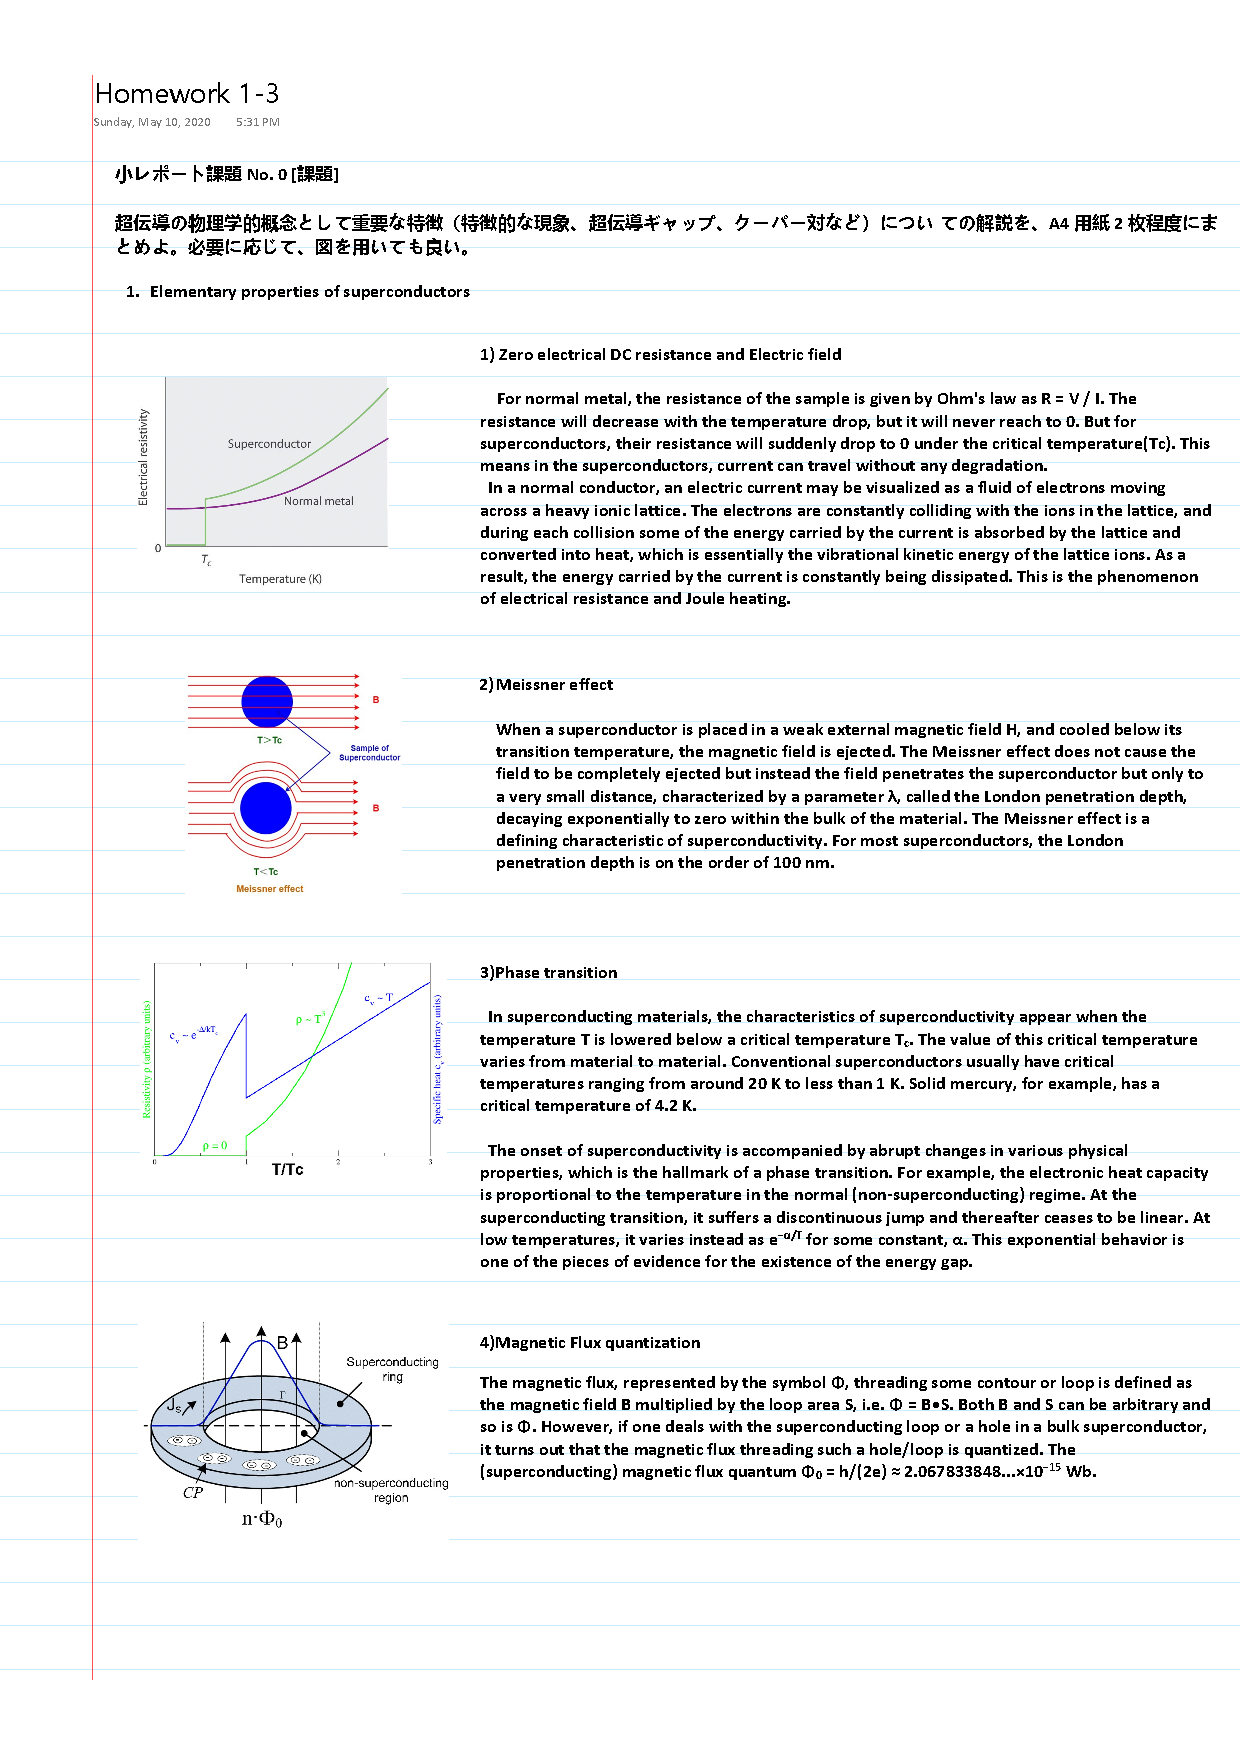
\includepdf[pages={1-3},scale=1]{Material Science Homework.pdf}
%---------------------------------第二题--------------------------------------
%\newpage
\question
\textbf{[問題 3.2]
\\フェルミ粒子の 2 粒子系について、反対称性 Φ(r1, r2) = −Φ(r2, r1) より次のことを示せ。
\\(ア). 式 (12) において、C1 = −C2 となることを示せ。そして、式 (13) も考慮して、式 (20) を導出せよ。
\\(イ). 式 (14) において、C = 0 となることを示せ。}\\
\\Answer:\\\\
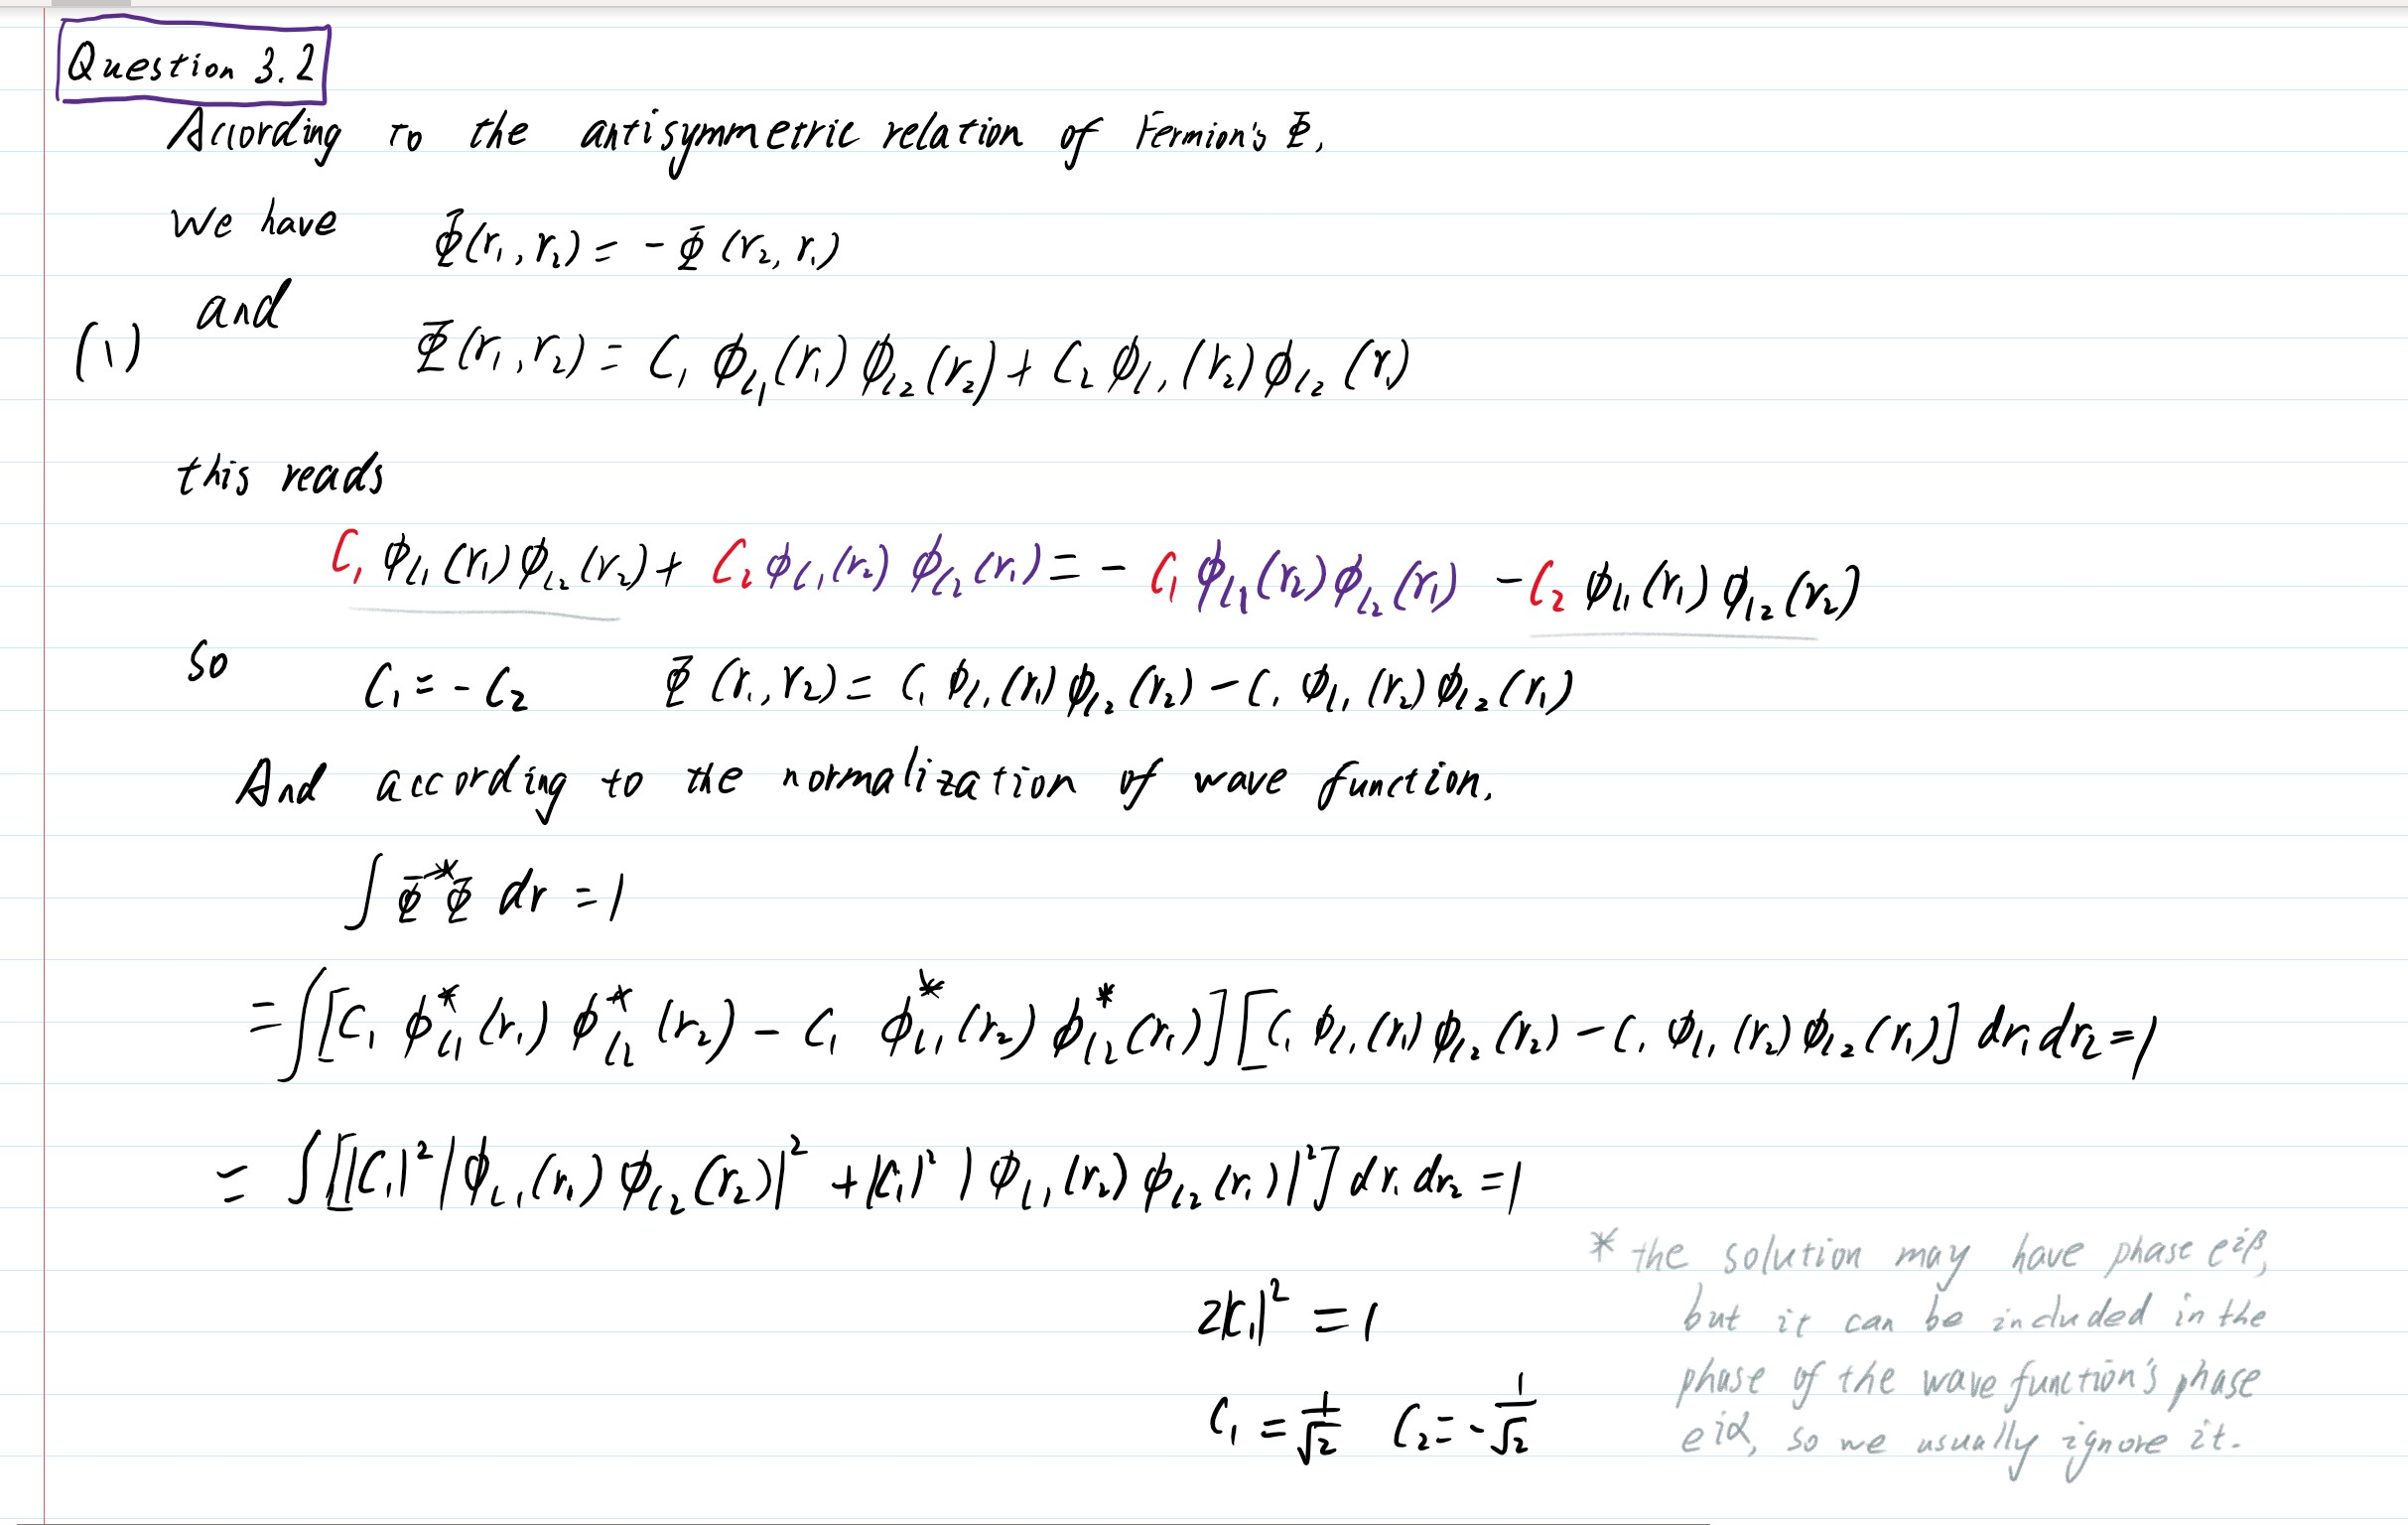
\includegraphics[scale=0.5]{Question/Q3.2.jpg}\\\\
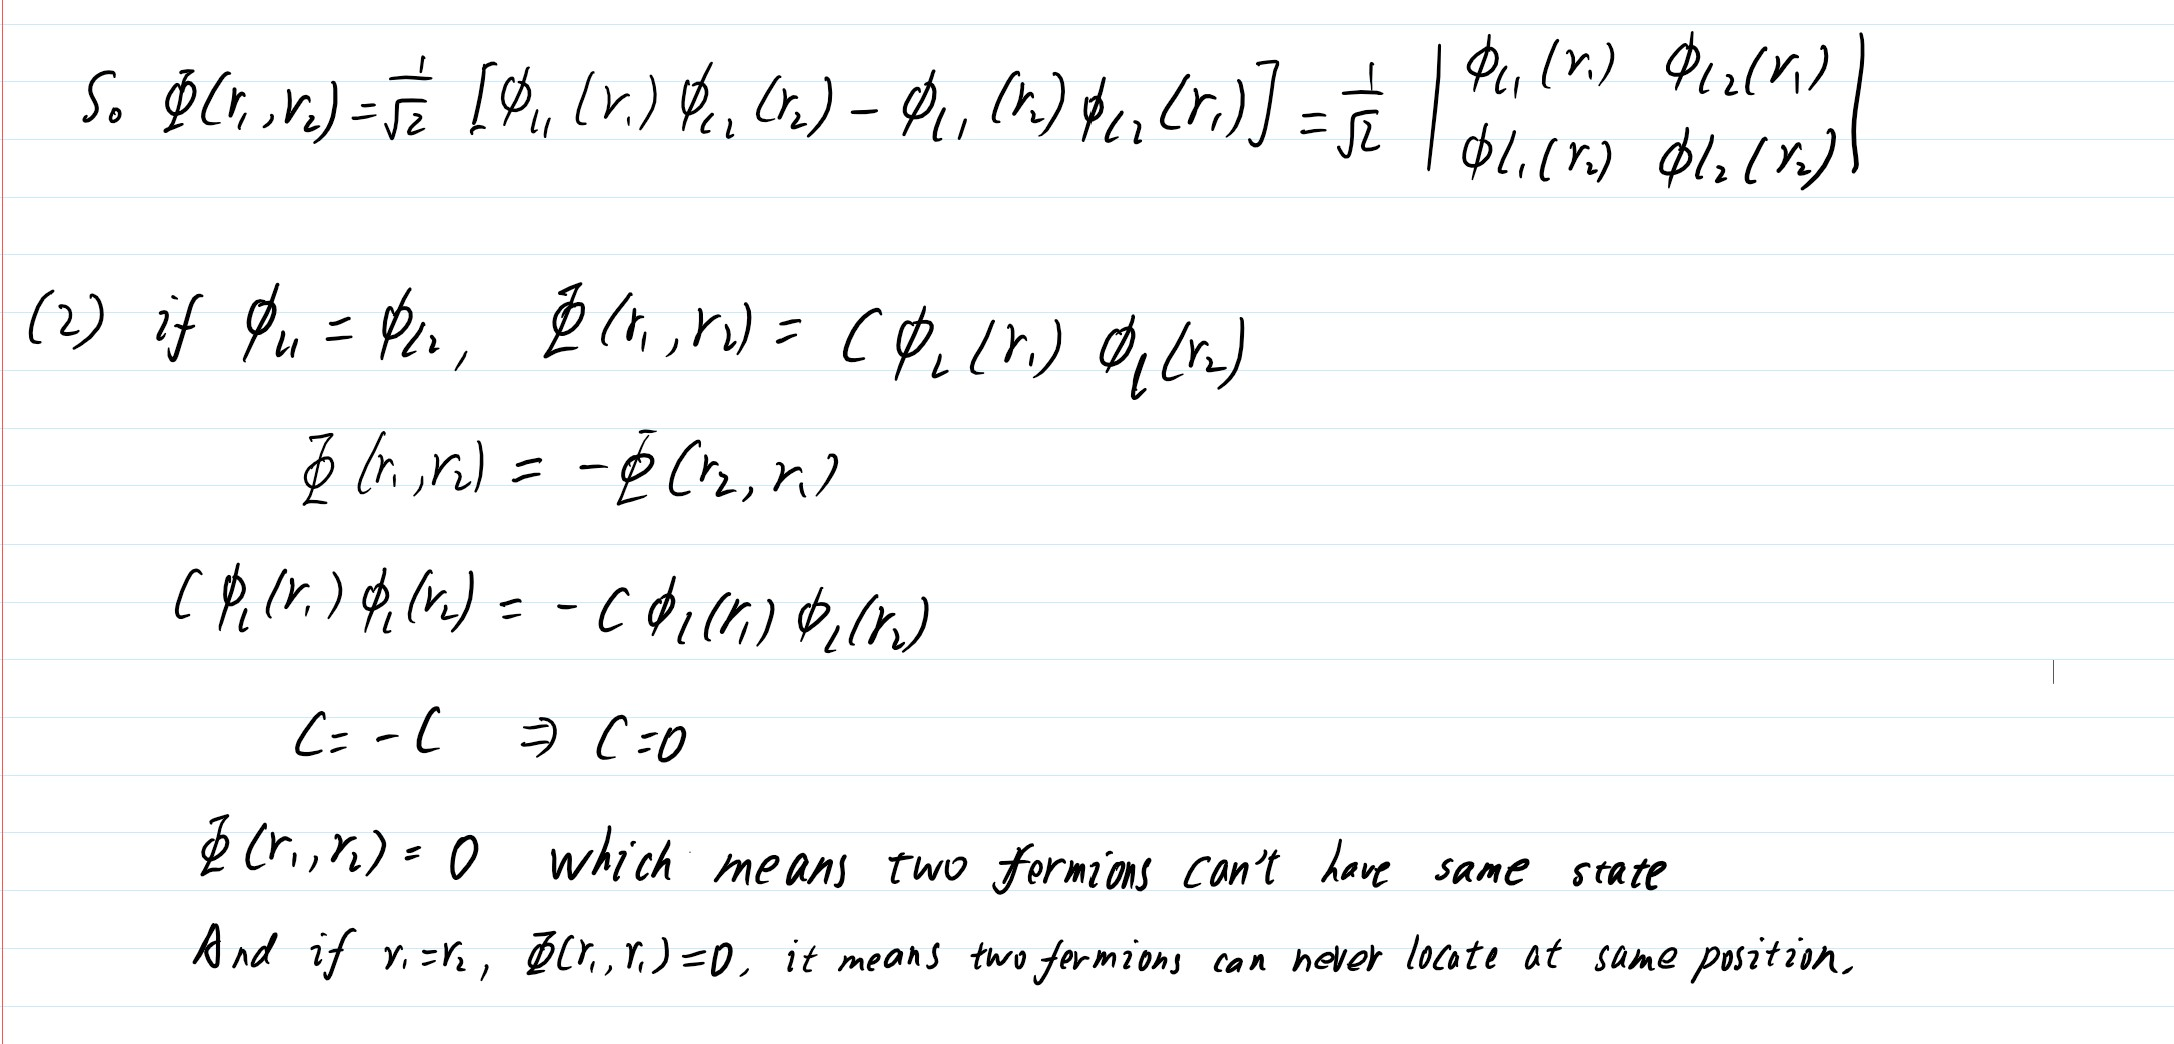
\includegraphics[scale=0.5]{Question/Q3.2-02.jpg}
% Sometimes questions get separated from their bodies. Use a \newpage to force
% them to wrap to the next page.
\newpage
\question
\textbf{[問題 3.6] フェルミ粒子 2 個の系において、1 粒子演算子がスレーター行列式に作用する時、式 (27)\\ の関係が成り立つことを証明せよ。}\\
\newline
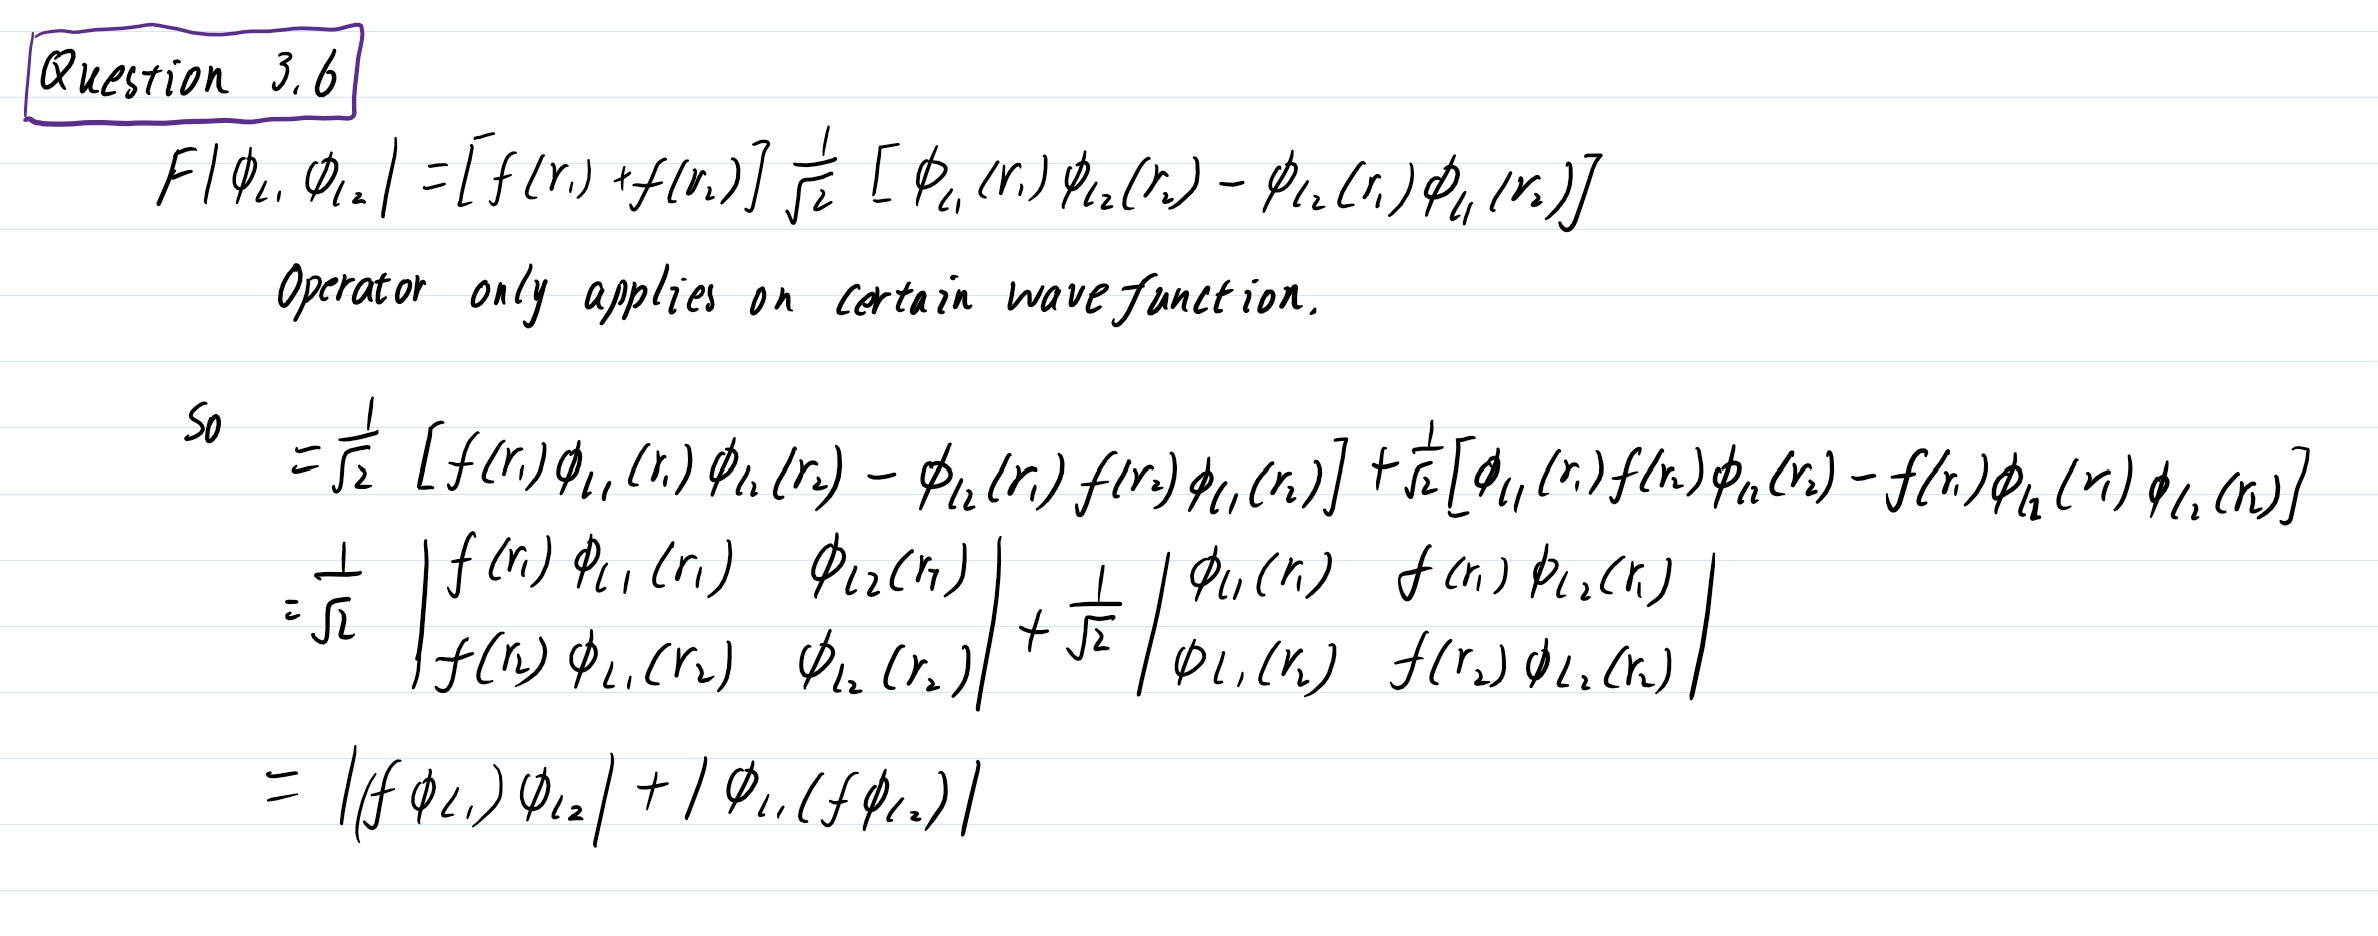
\includegraphics[scale=0.5]{Question/Q3.6.jpg}
\newpage
\question
\textbf{[問題 3.10]\\(ア). 生成・消滅演算子が作用した次の (a)-(d) の状態を計算して答えよ。\\
(イ). (ア) の結果より、以下の、µ = v の場合の反交換関係 (a)-(c)、および、数演算子に関する関係式 (d) が成り立つことを示せ.}
\newline
\\
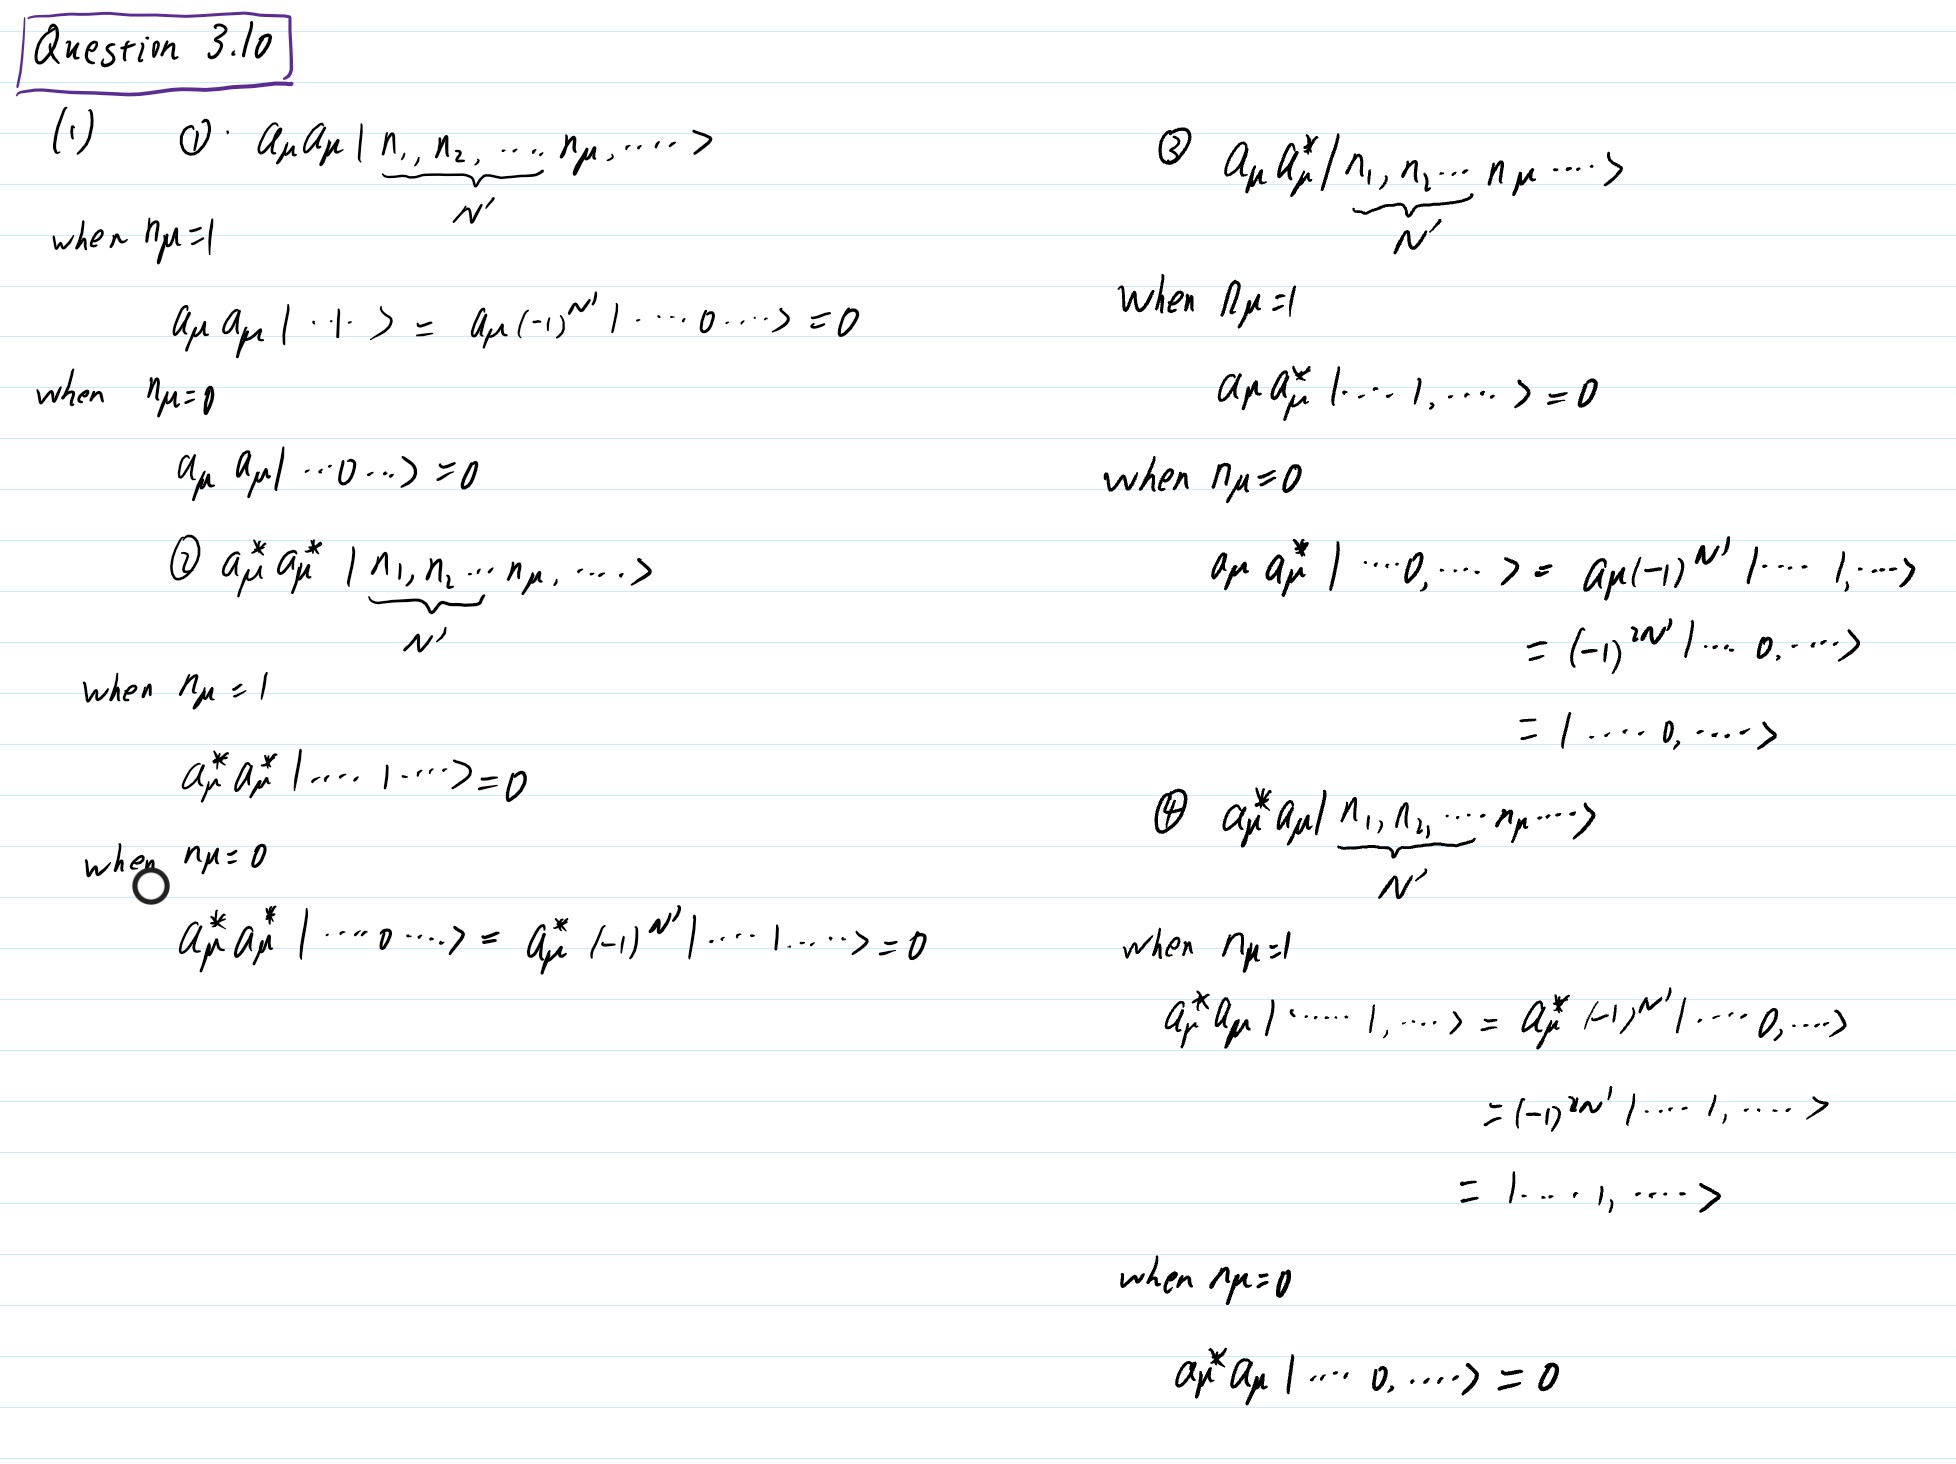
\includegraphics[scale=0.6]{Question/Q3.10-1.jpg}
\newline
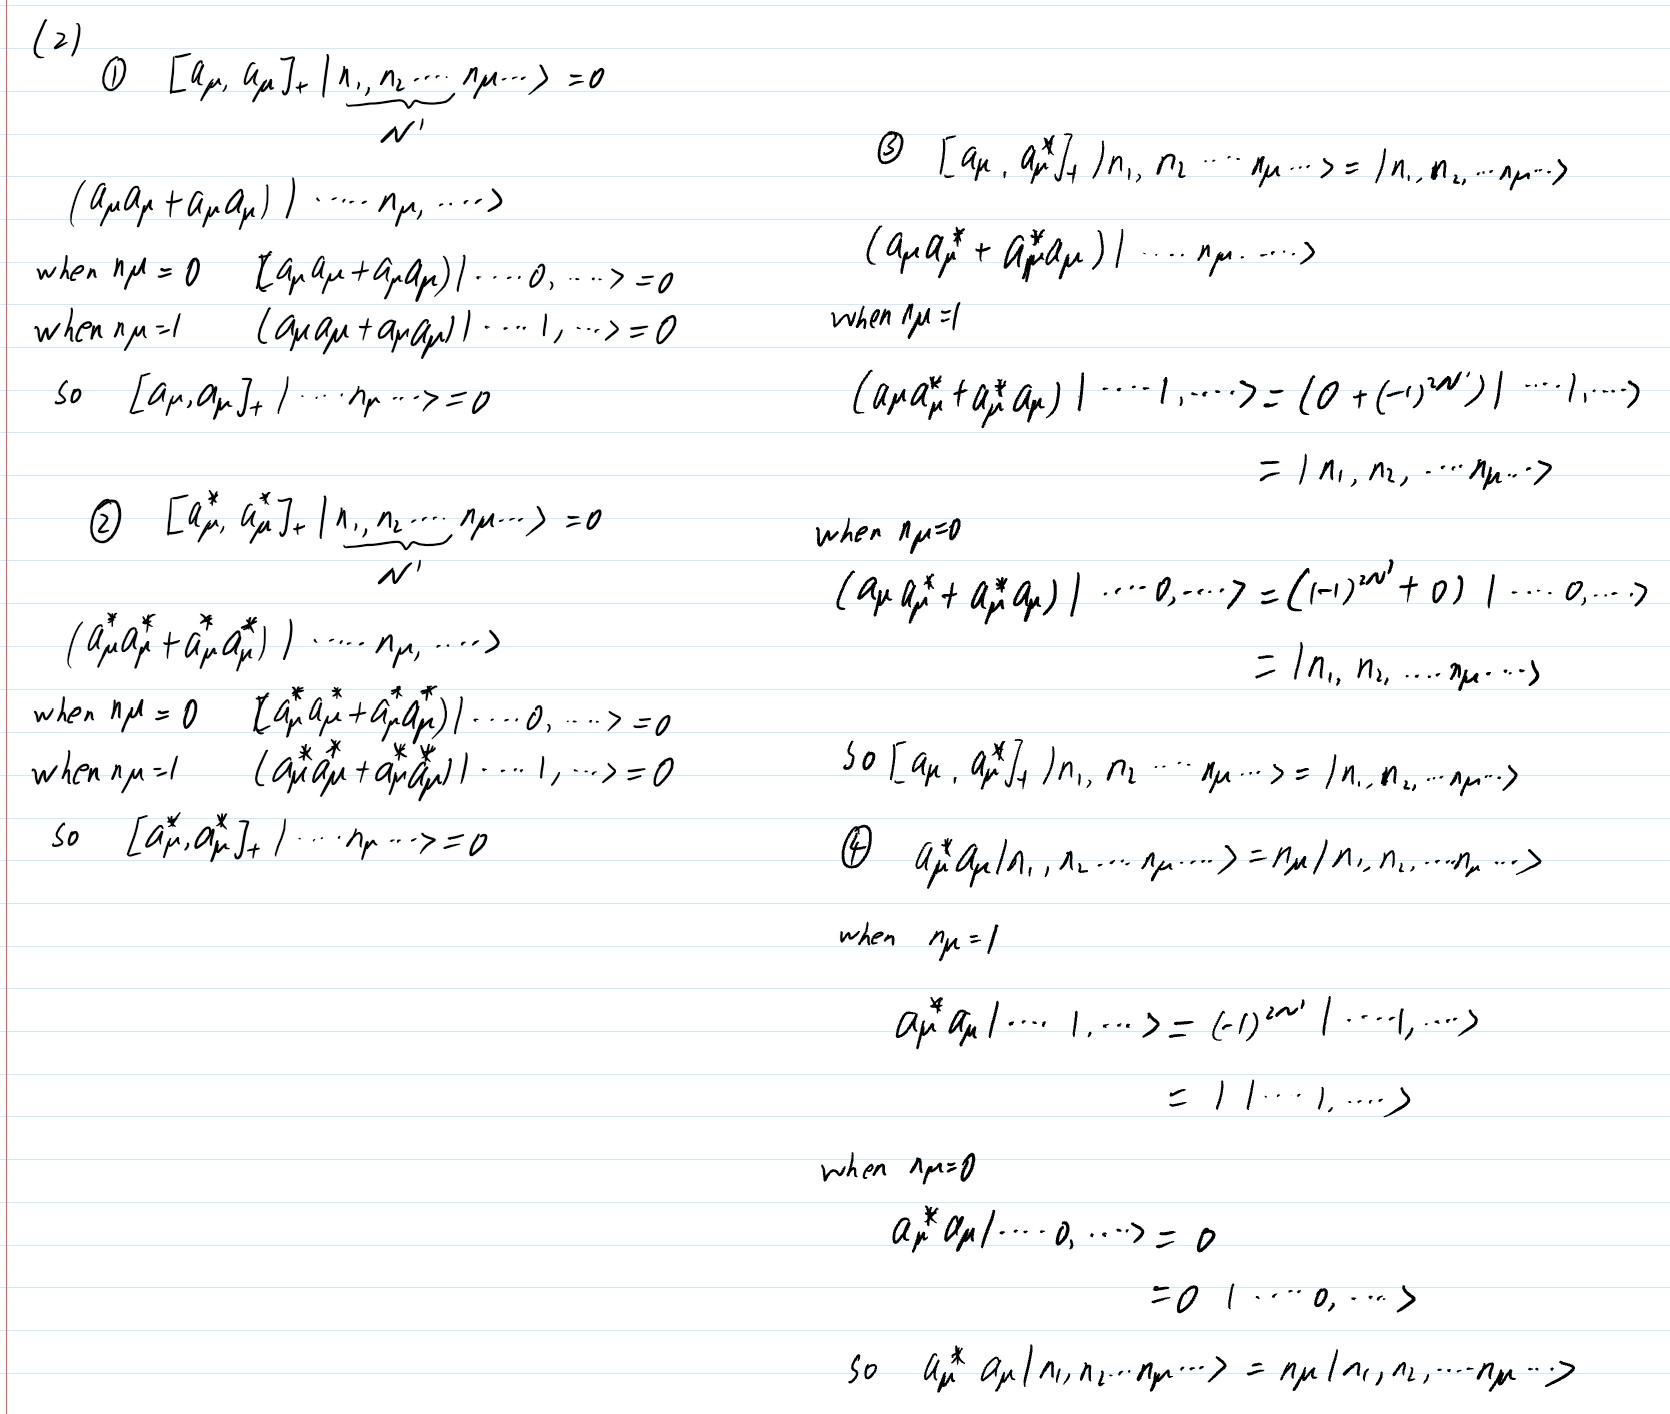
\includegraphics[scale=0.8]{Question/Q3.10-2.jpg}
\newpage
\question
\textbf{[問題 3.16]\\場の演算子の反交換関係・交換関係の式 (51) と (52) と (53) の3つの関係式が成り立つことを証明せよ。}\\
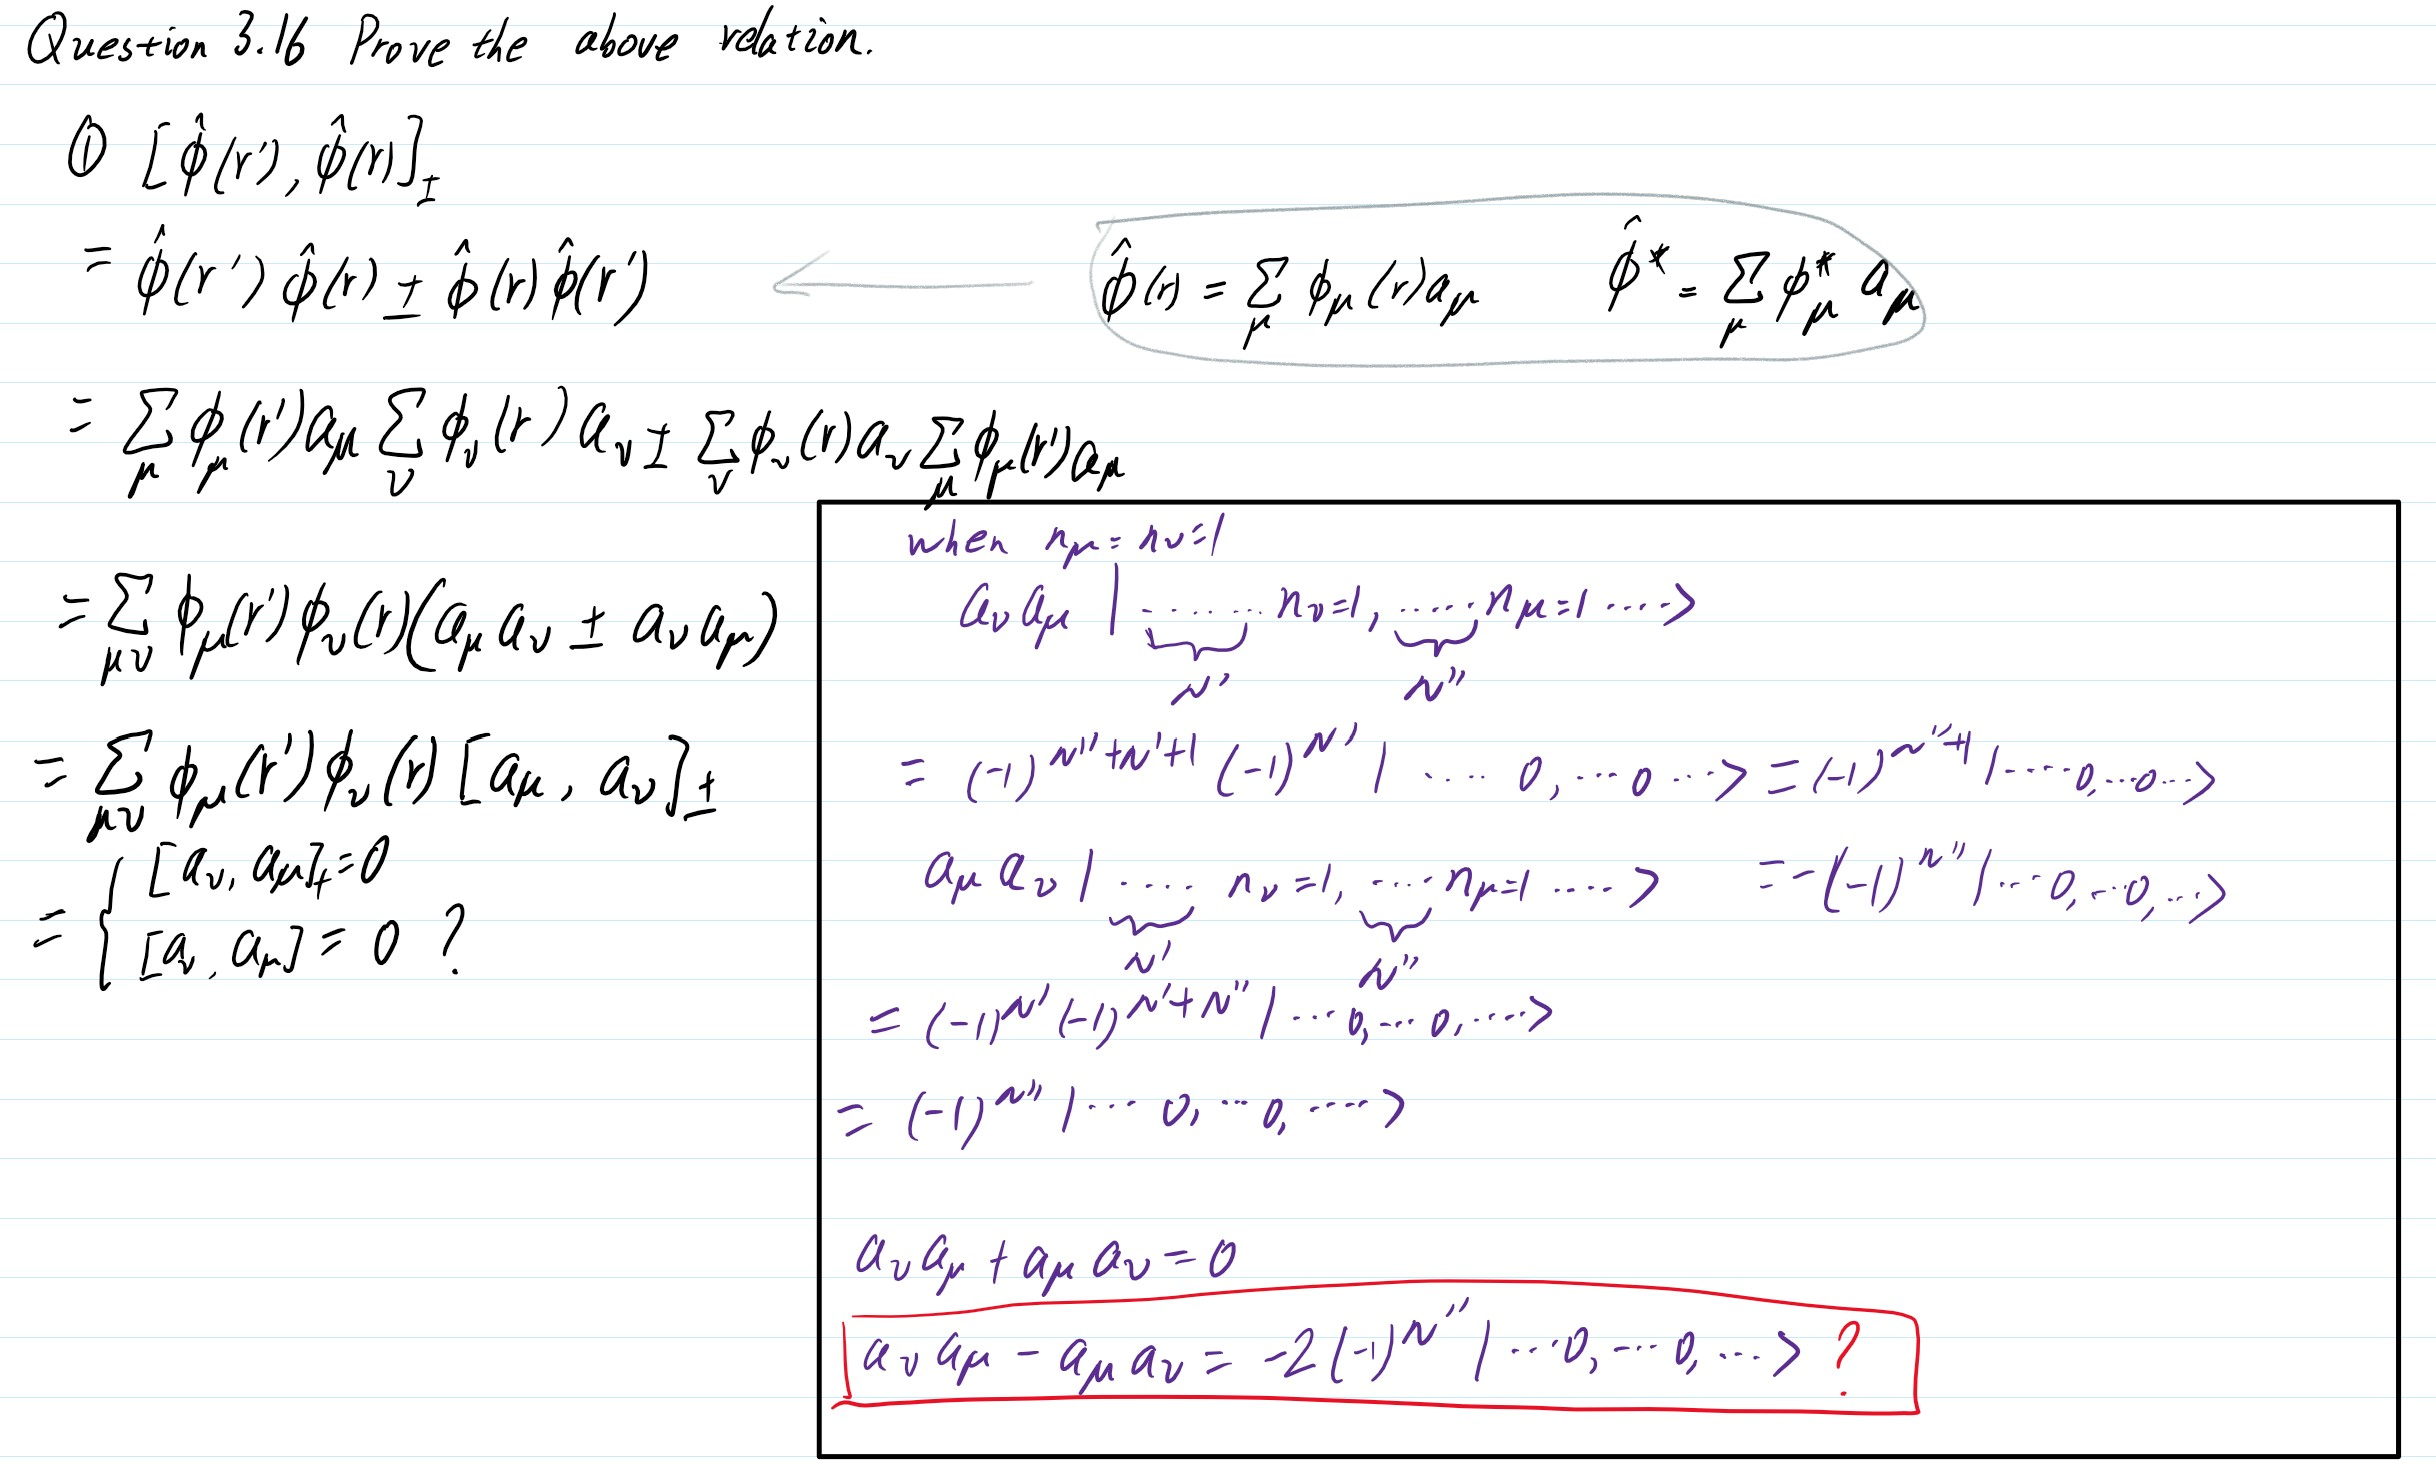
\includegraphics[scale=0.6]{Question/Q3.16-1.jpg}\\
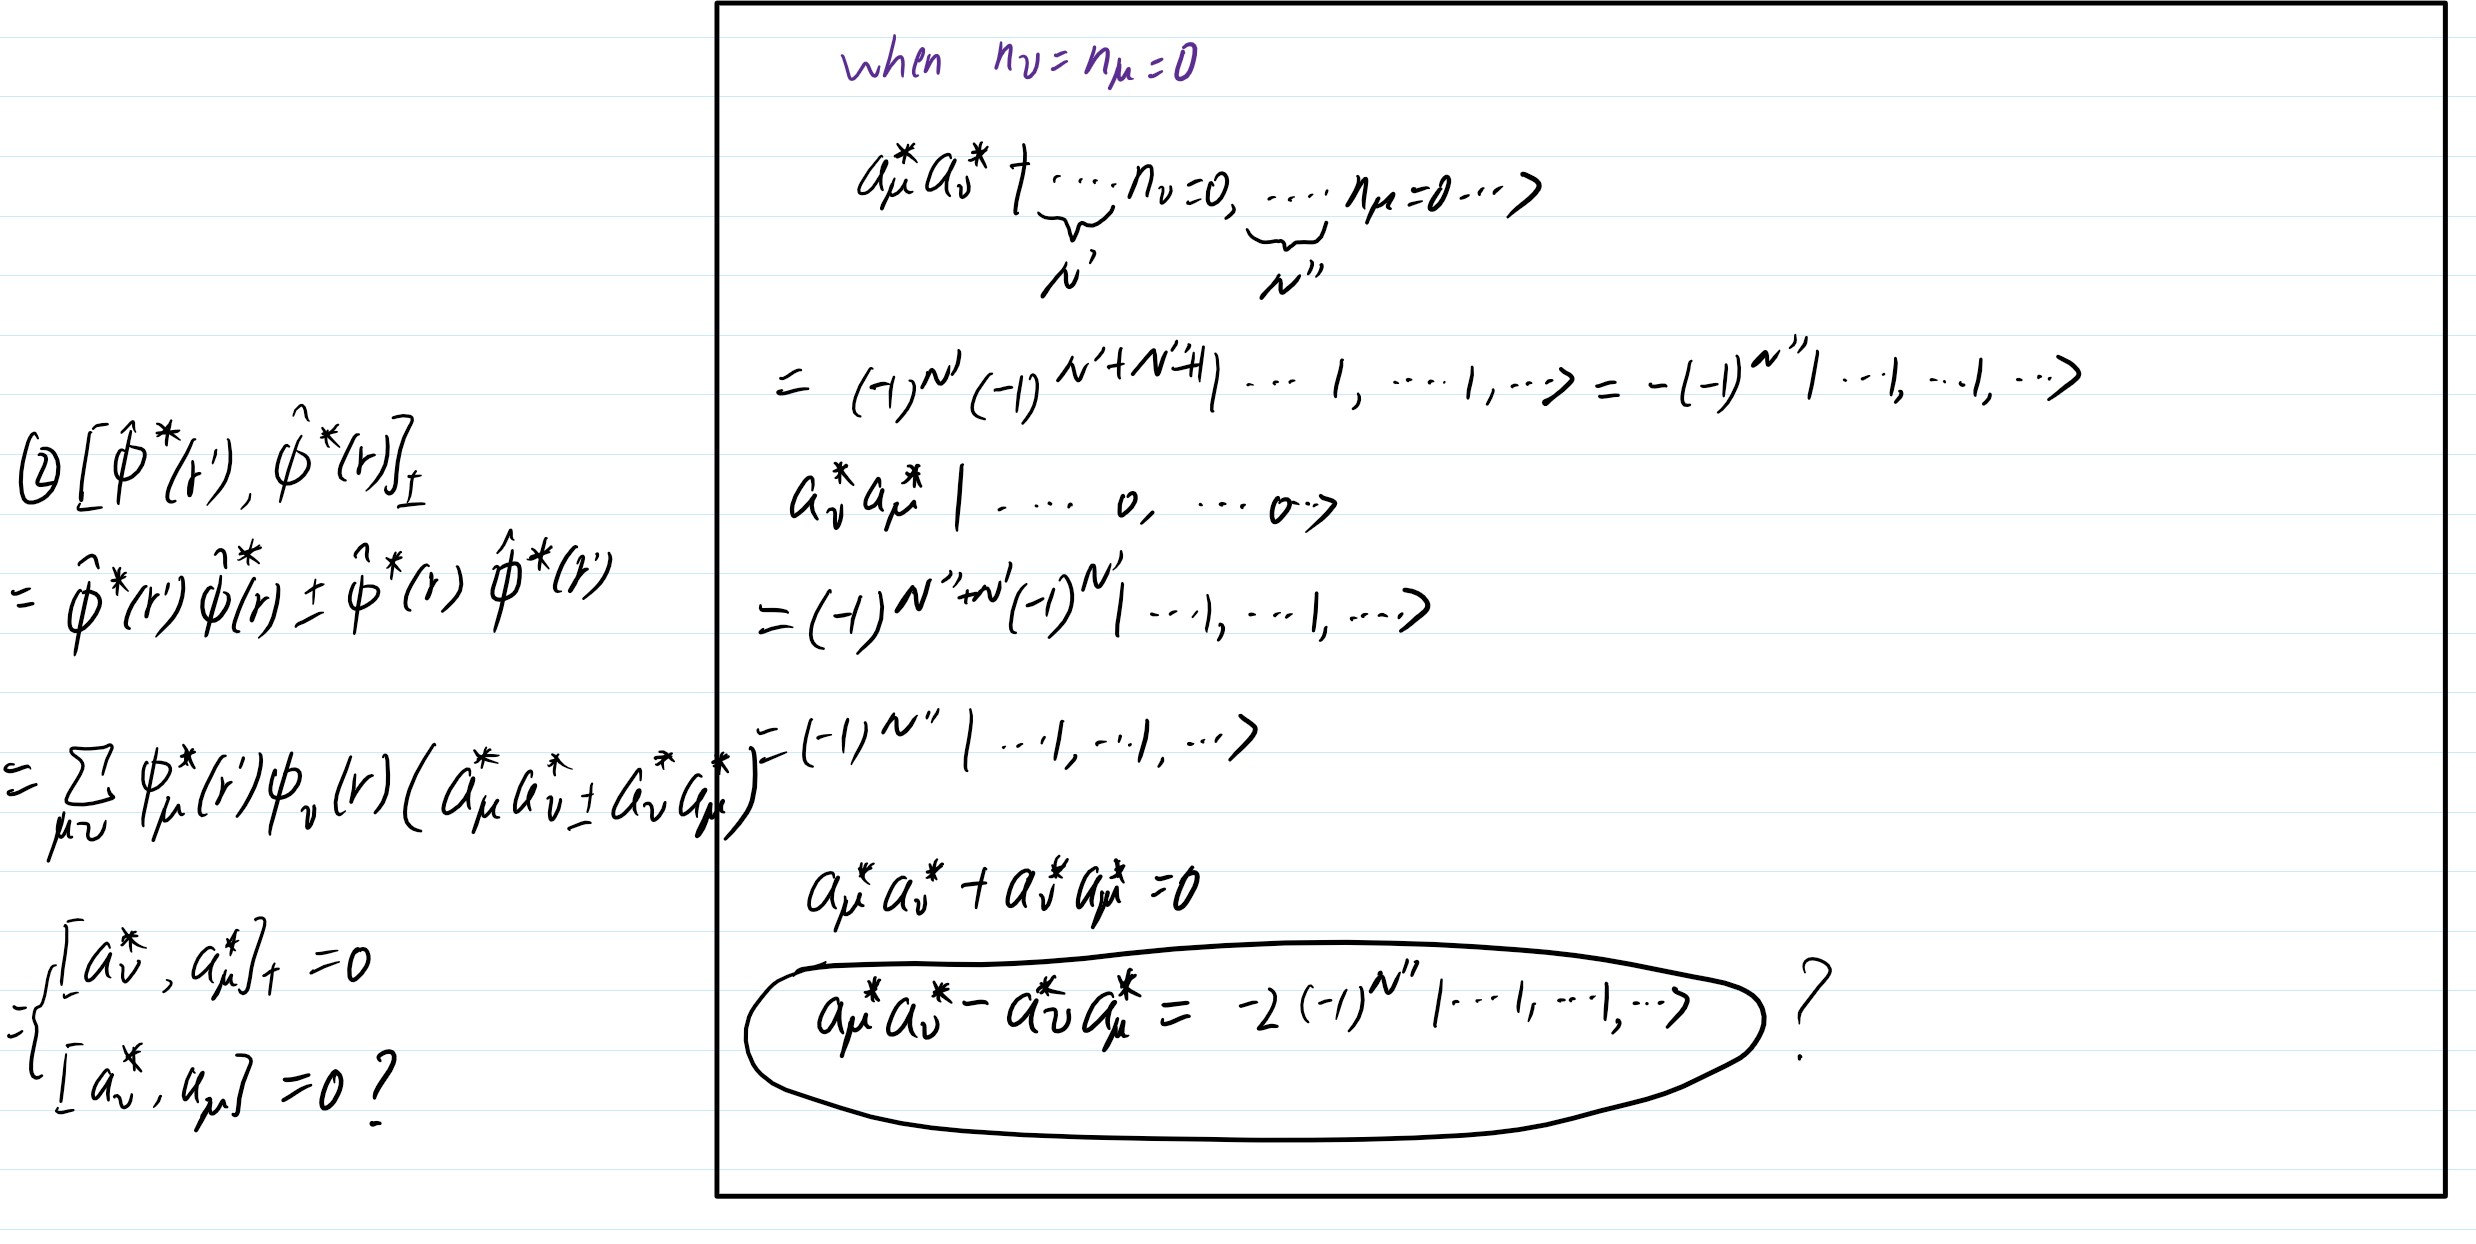
\includegraphics[scale=0.6]{Question/Q3.16-2.jpg}\\
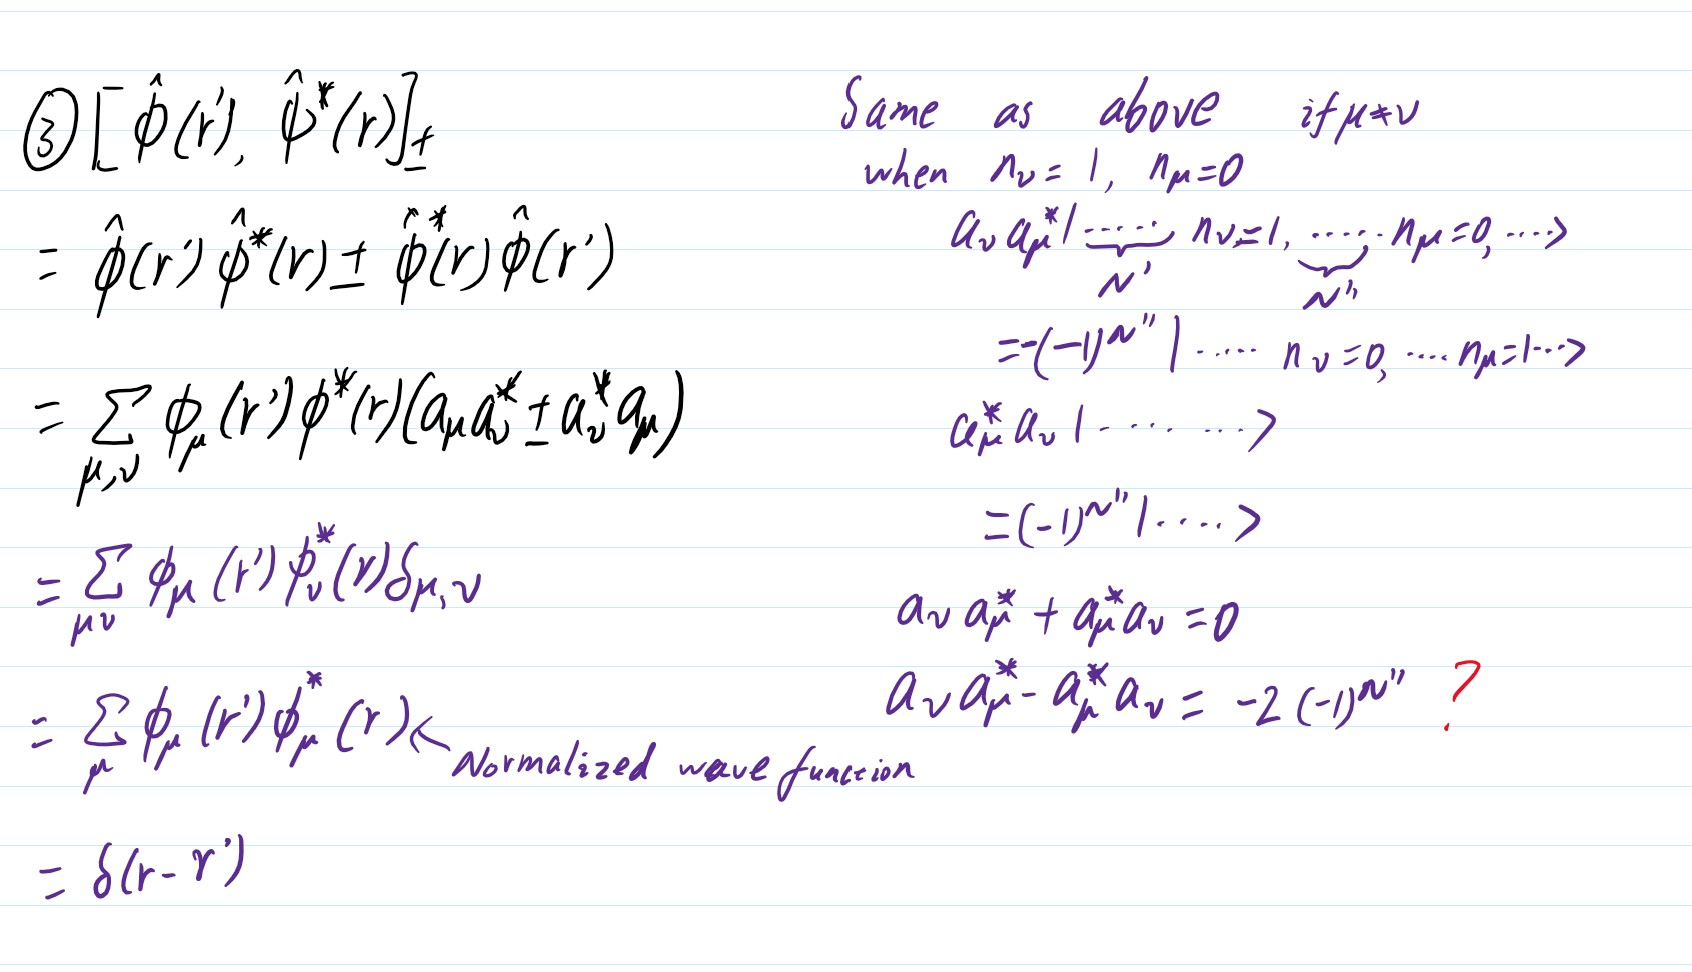
\includegraphics[scale=0.6]{Question/Q3.16-3.jpg}
\newpage
\question
\textbf{[問題 3.24]\\式 (79) と式 (81) の導出を示せ。}\\
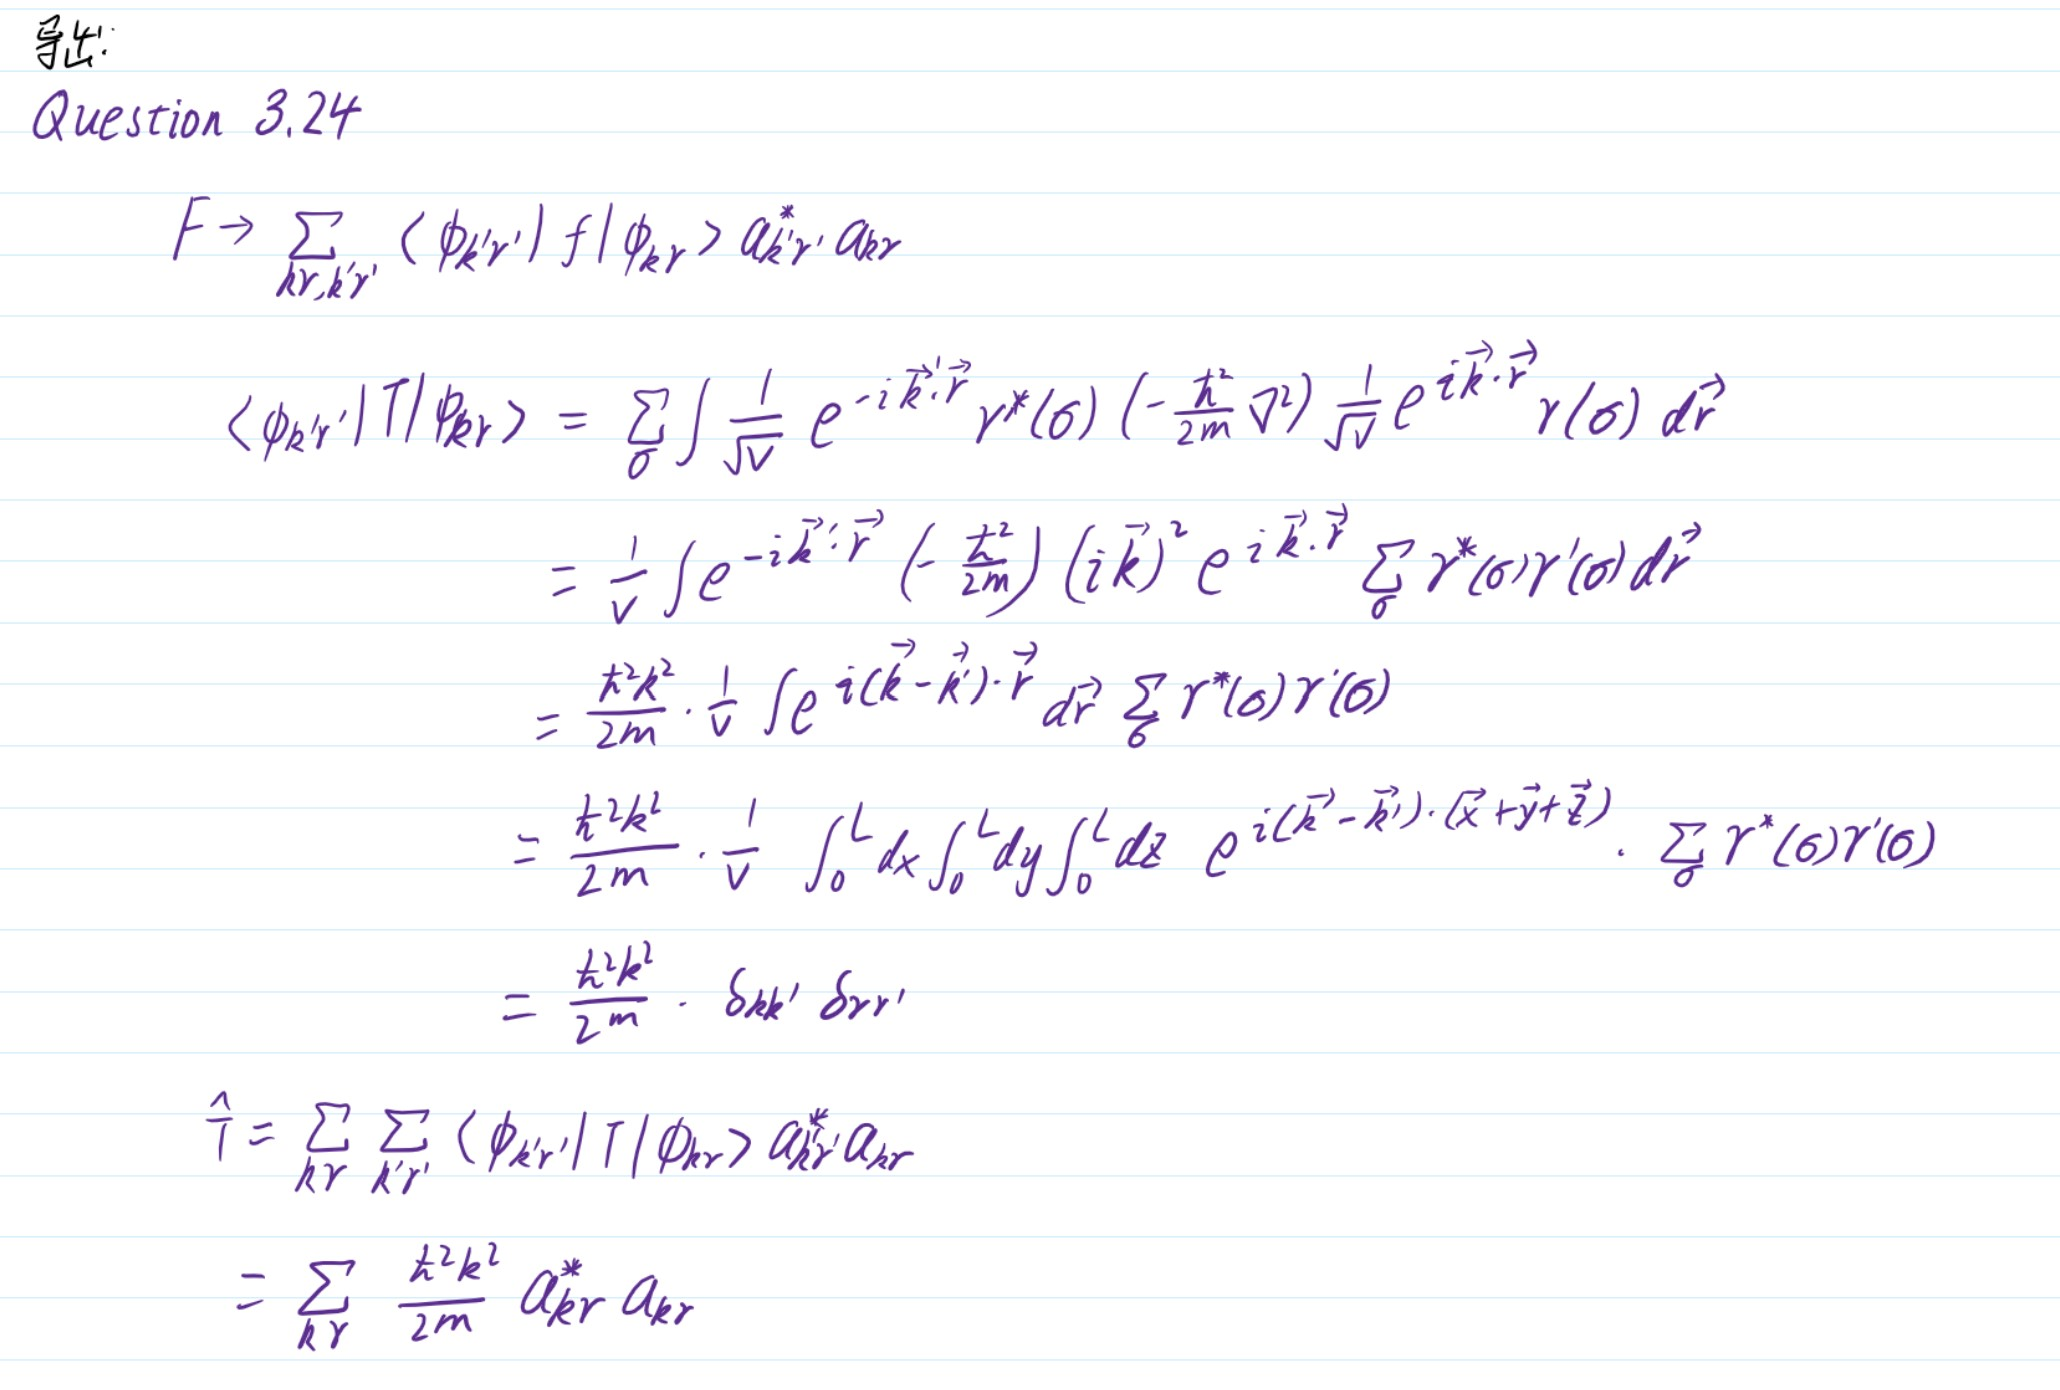
\includegraphics[scale=0.7]{Question/Q3.24-1.jpg}\\
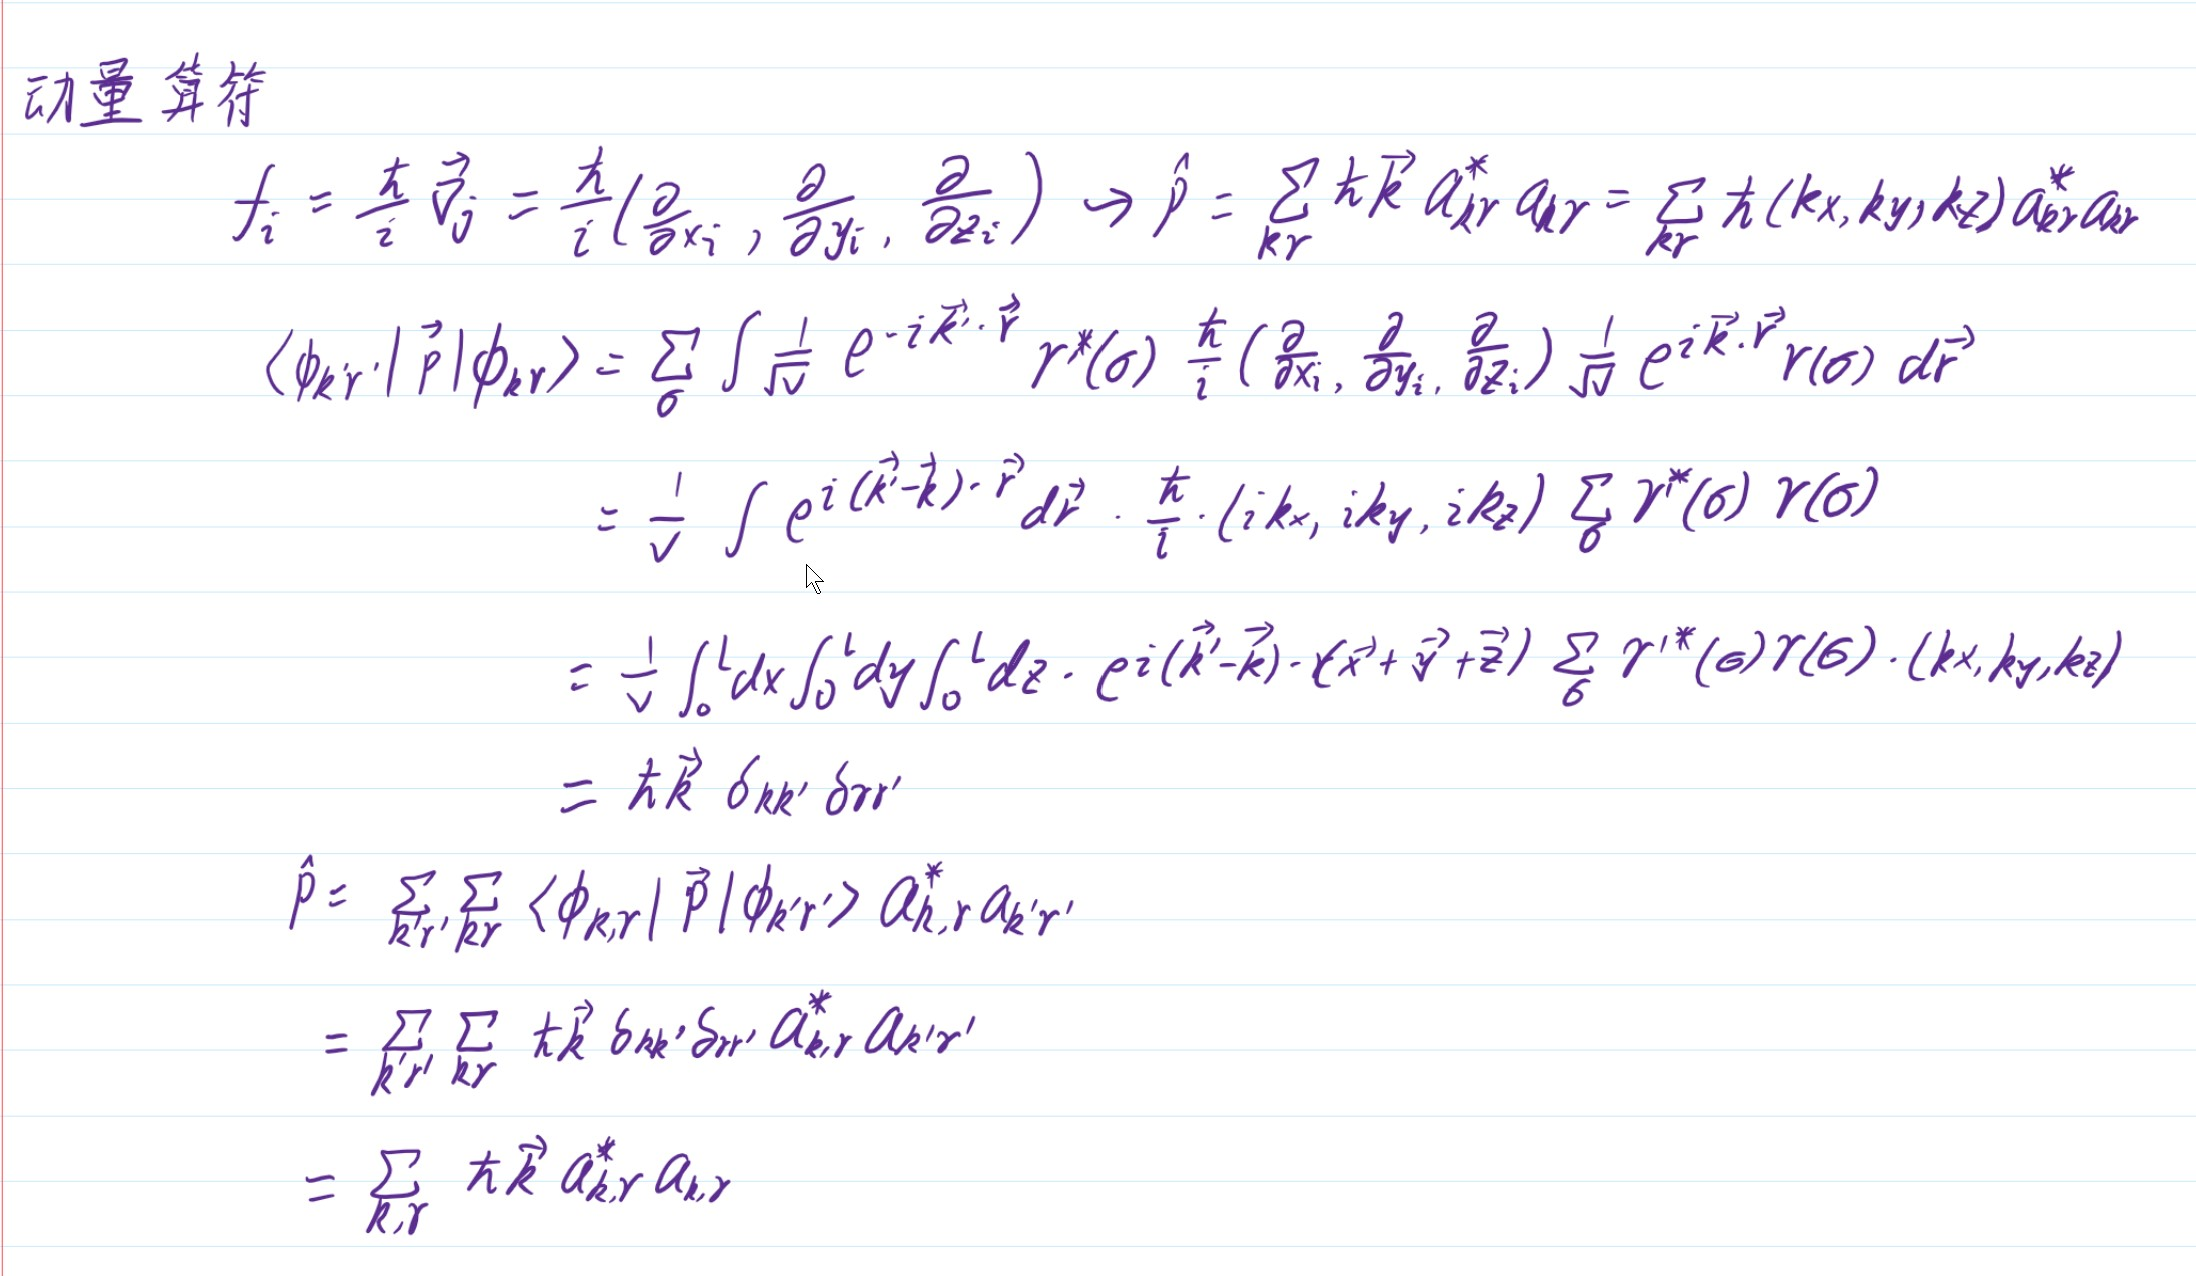
\includegraphics[scale=0.6]{Question/Q3.24-2.jpg}
\newpage
\question
\textbf{[問題 3.25]\\2 粒子間の相互作用 g(ri − rj ) が式 (85) のように与えられる場合に式 (84) を計算し、式 (86) を導出せよ。}\\
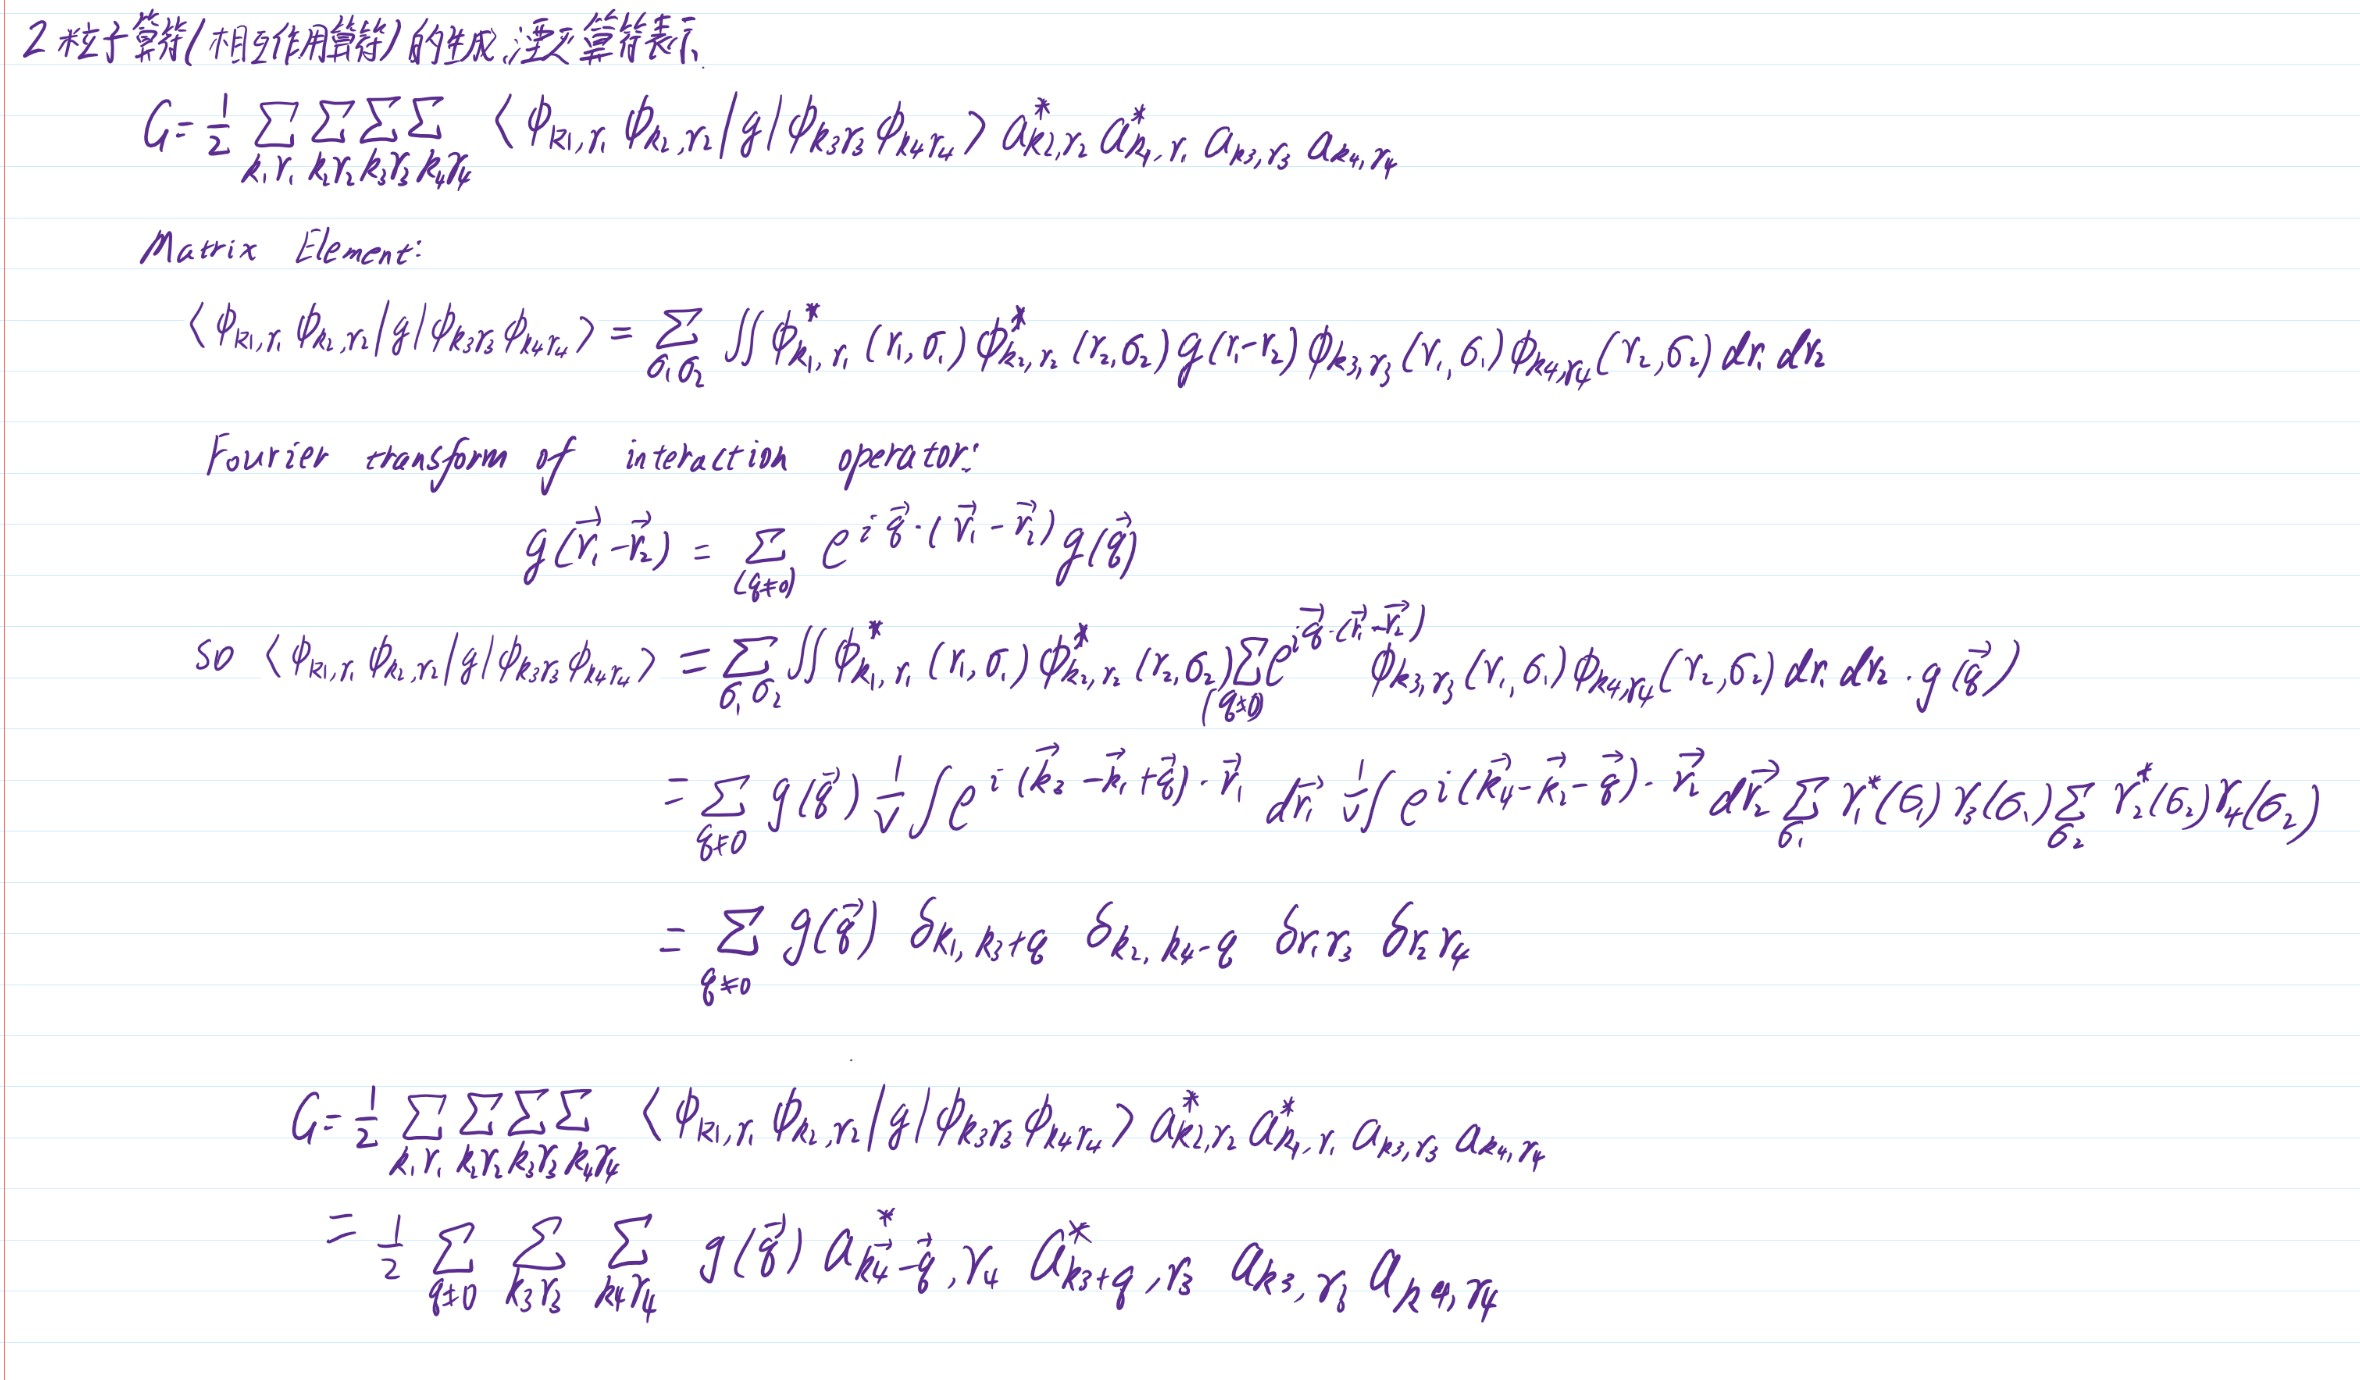
\includegraphics[scale=0.6]{Question/Q3.25.jpg}
\newpage
\question\textbf{小レポート課題 No.1\\
[問題 1]式 (102) で与えられる BCS 波動関数について、以下の問に答えよ。\\
(ア). 式 (104) の関係の導出を示し、|uk|2 + |vk|2 = 1 の条件が得られることを示せ。\\
(イ). 式 (106) の関係の導出を示せ。\\
(ウ). 式 (108) の関係の導出を示せ。\\
[問題2]式 (111) で与えられる ⟨E − µN⟩ の変分がゼロとなることより、次の関係が得られることを示せ。\\
(ア).BCS 波動関数に関して、|vk|2 と |uk|2 が式 (115) のように与えられることの導出を示せ。\\
(イ).無道着 (Self-consisitent) の条件が式 (116) のように与えられることの導出を示せ。}\\
\newpage
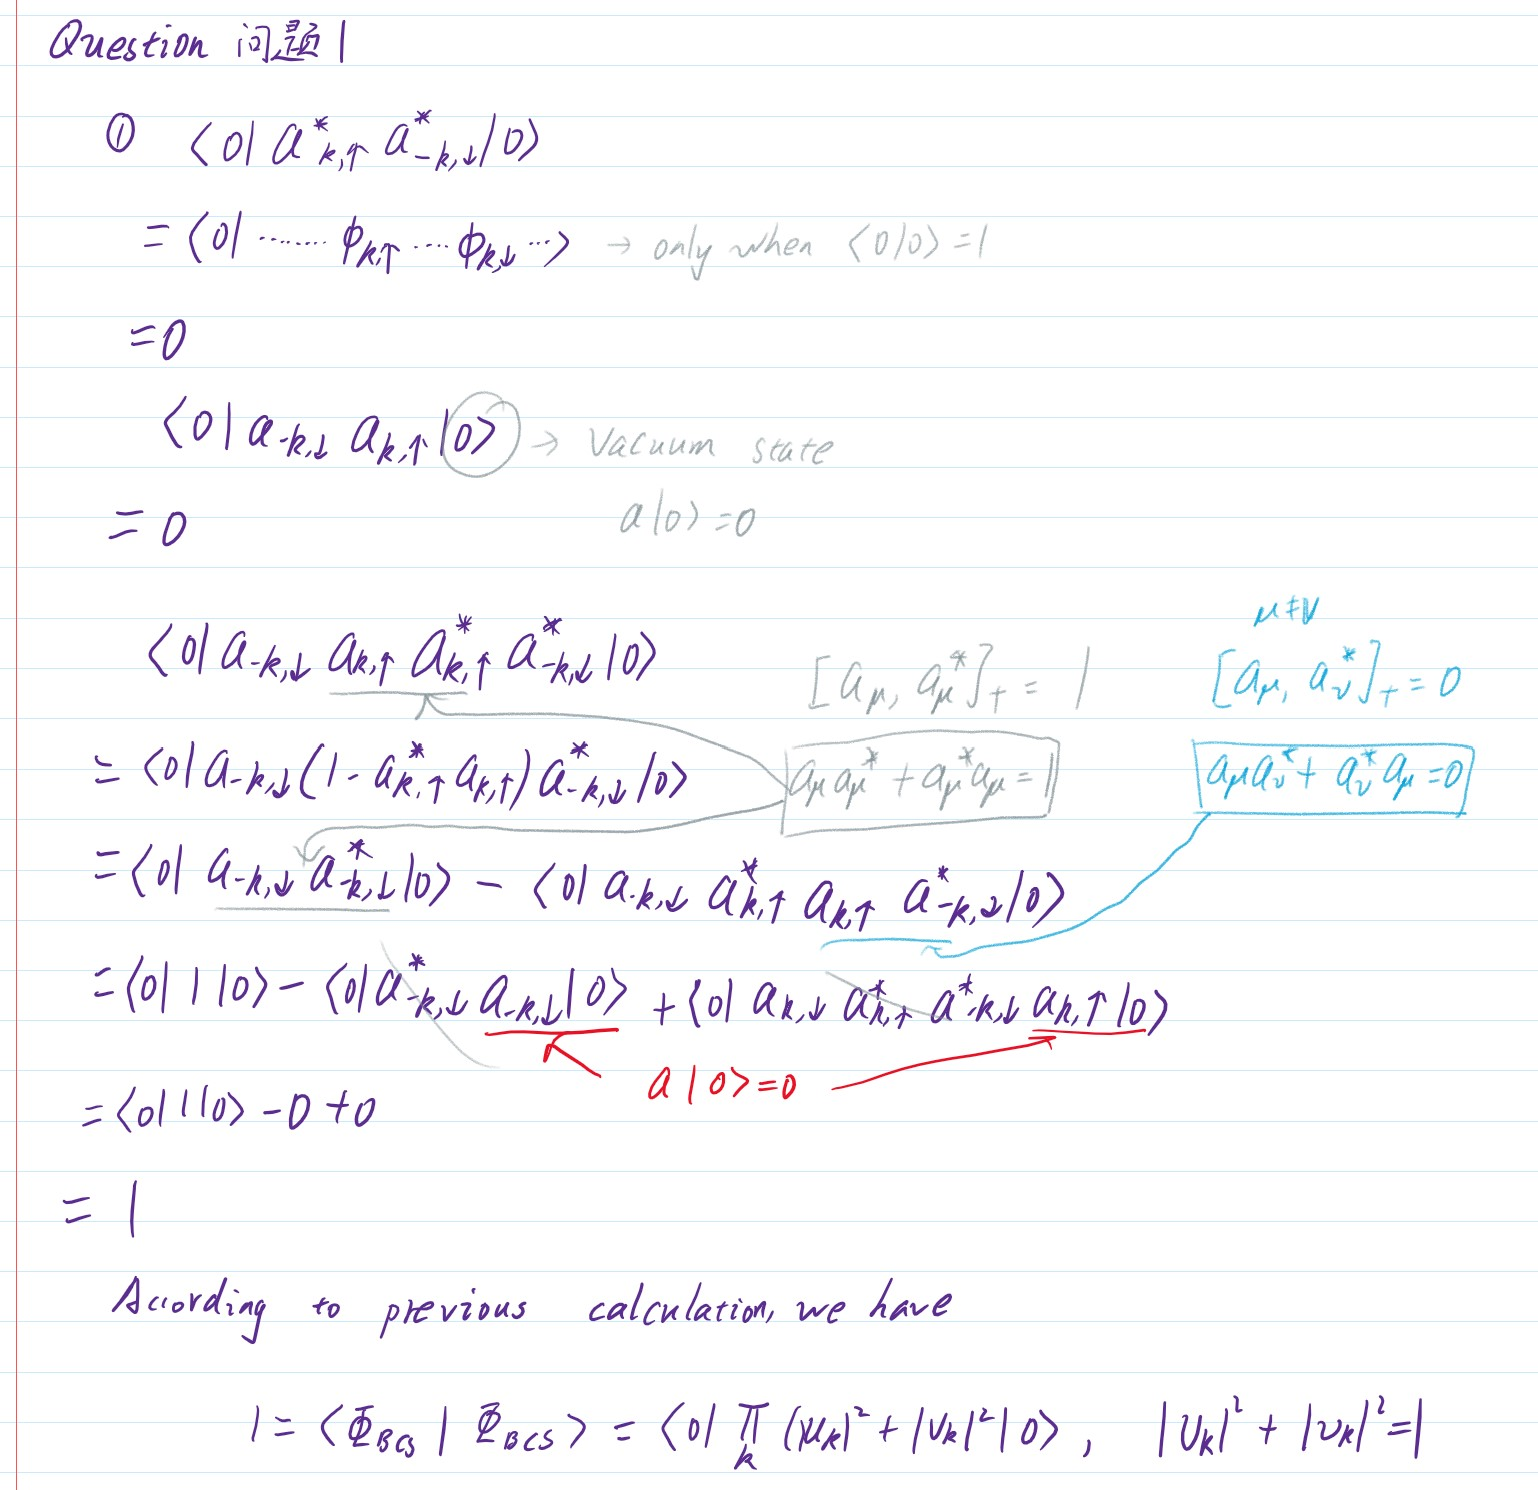
\includegraphics[scale=0.57]{Question/Task1-1.jpg}\\
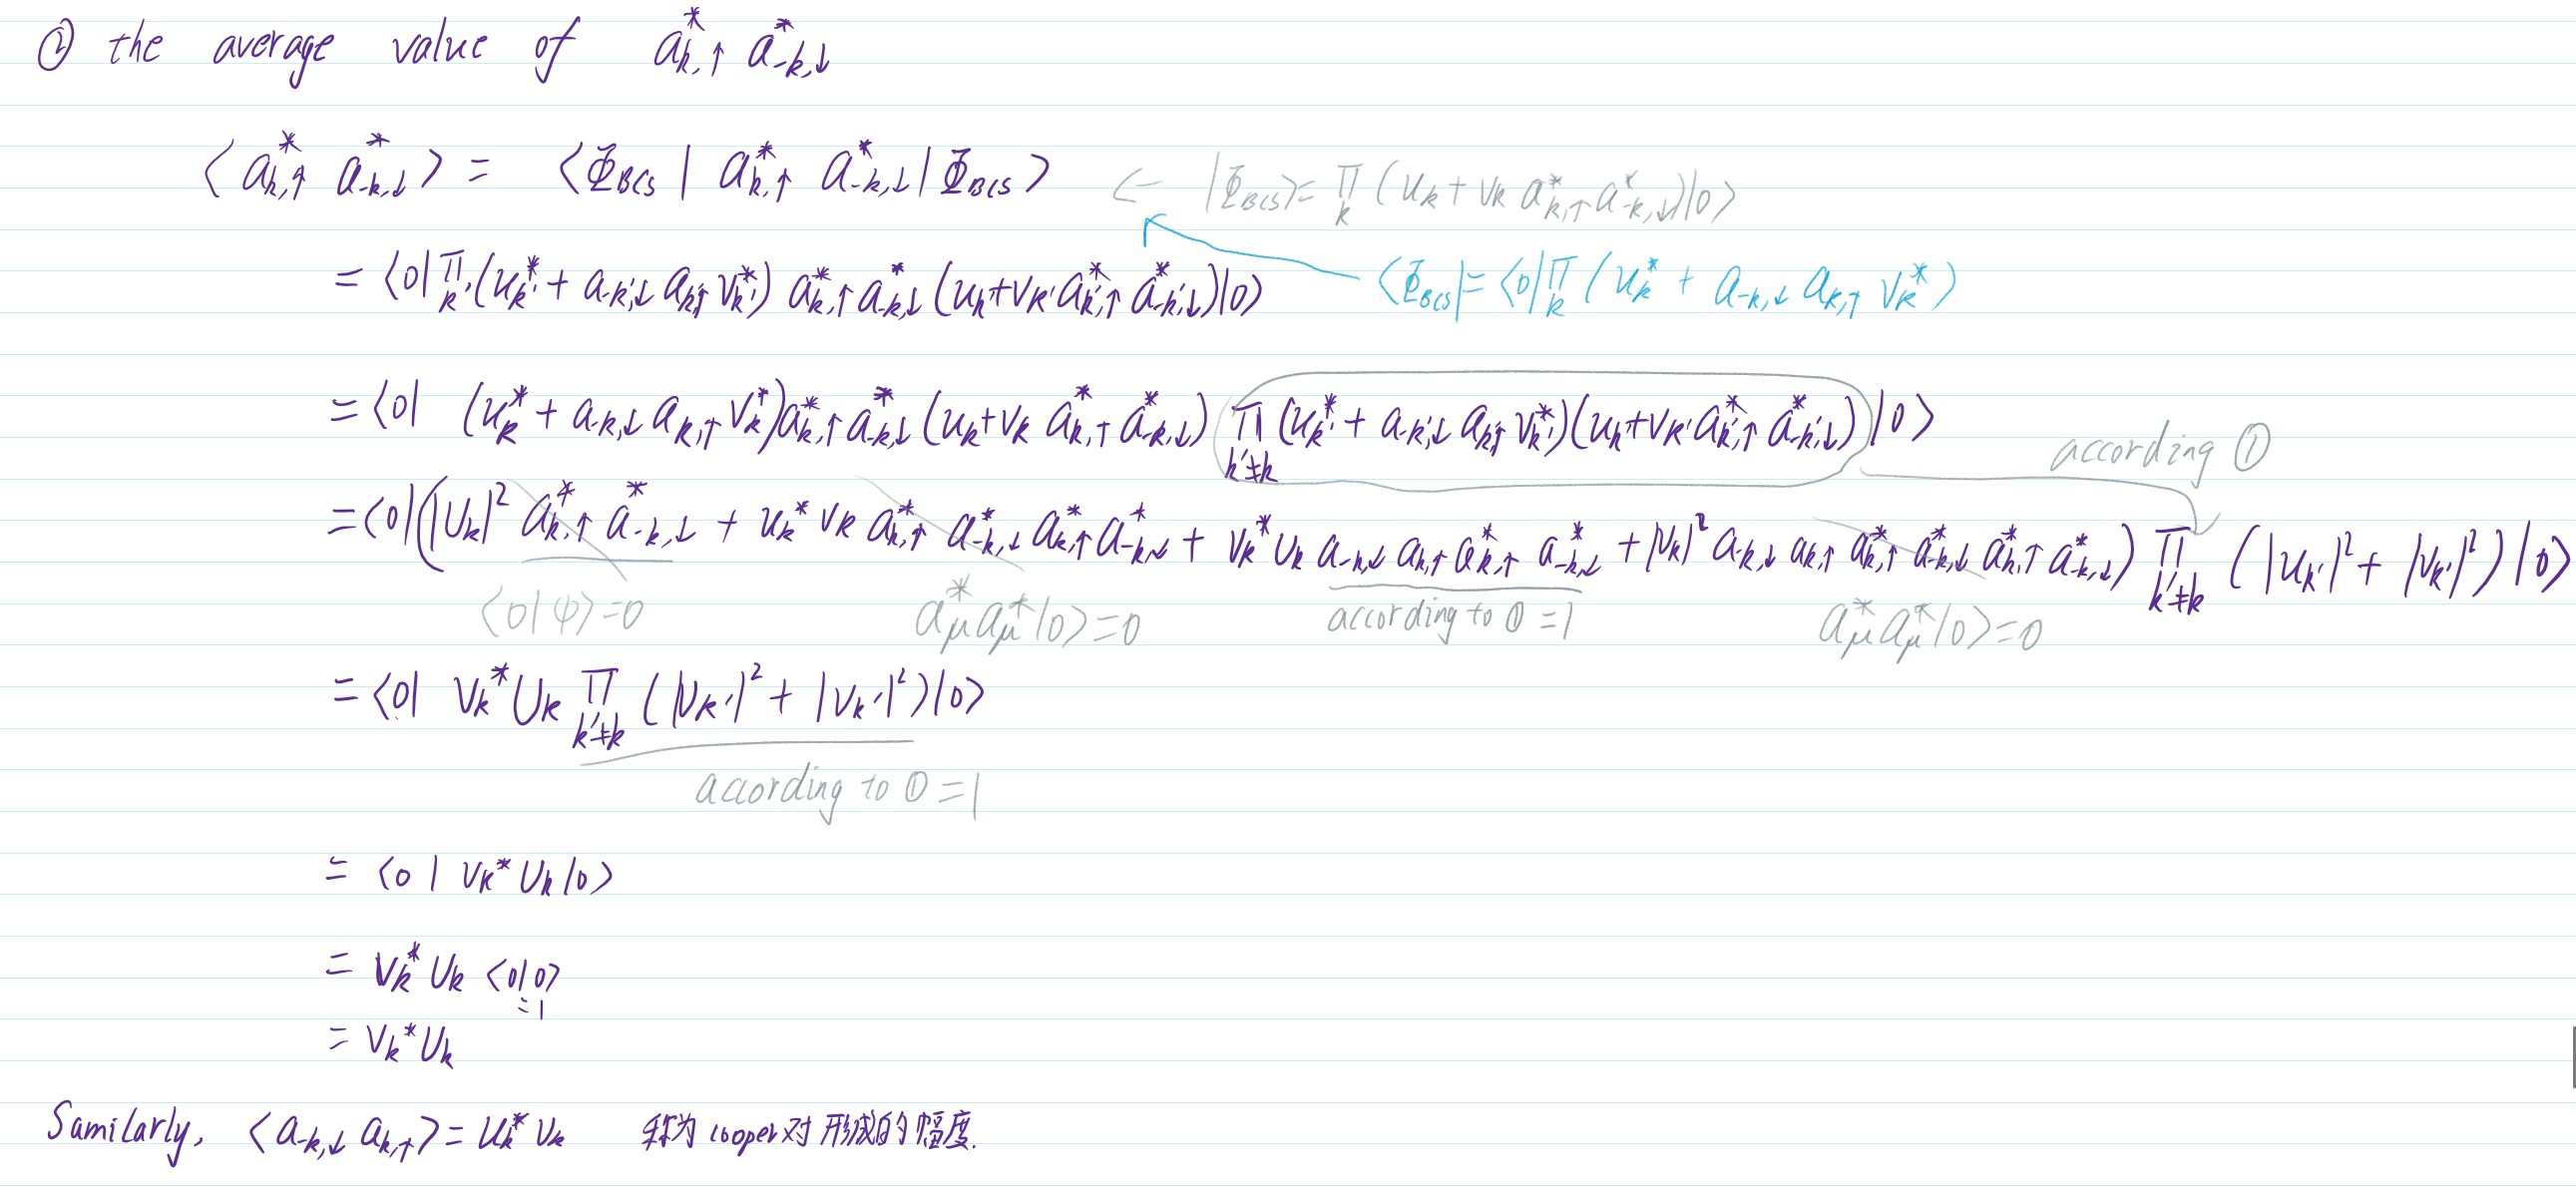
\includegraphics[scale=0.57]{Question/Task1-2.jpg}\\
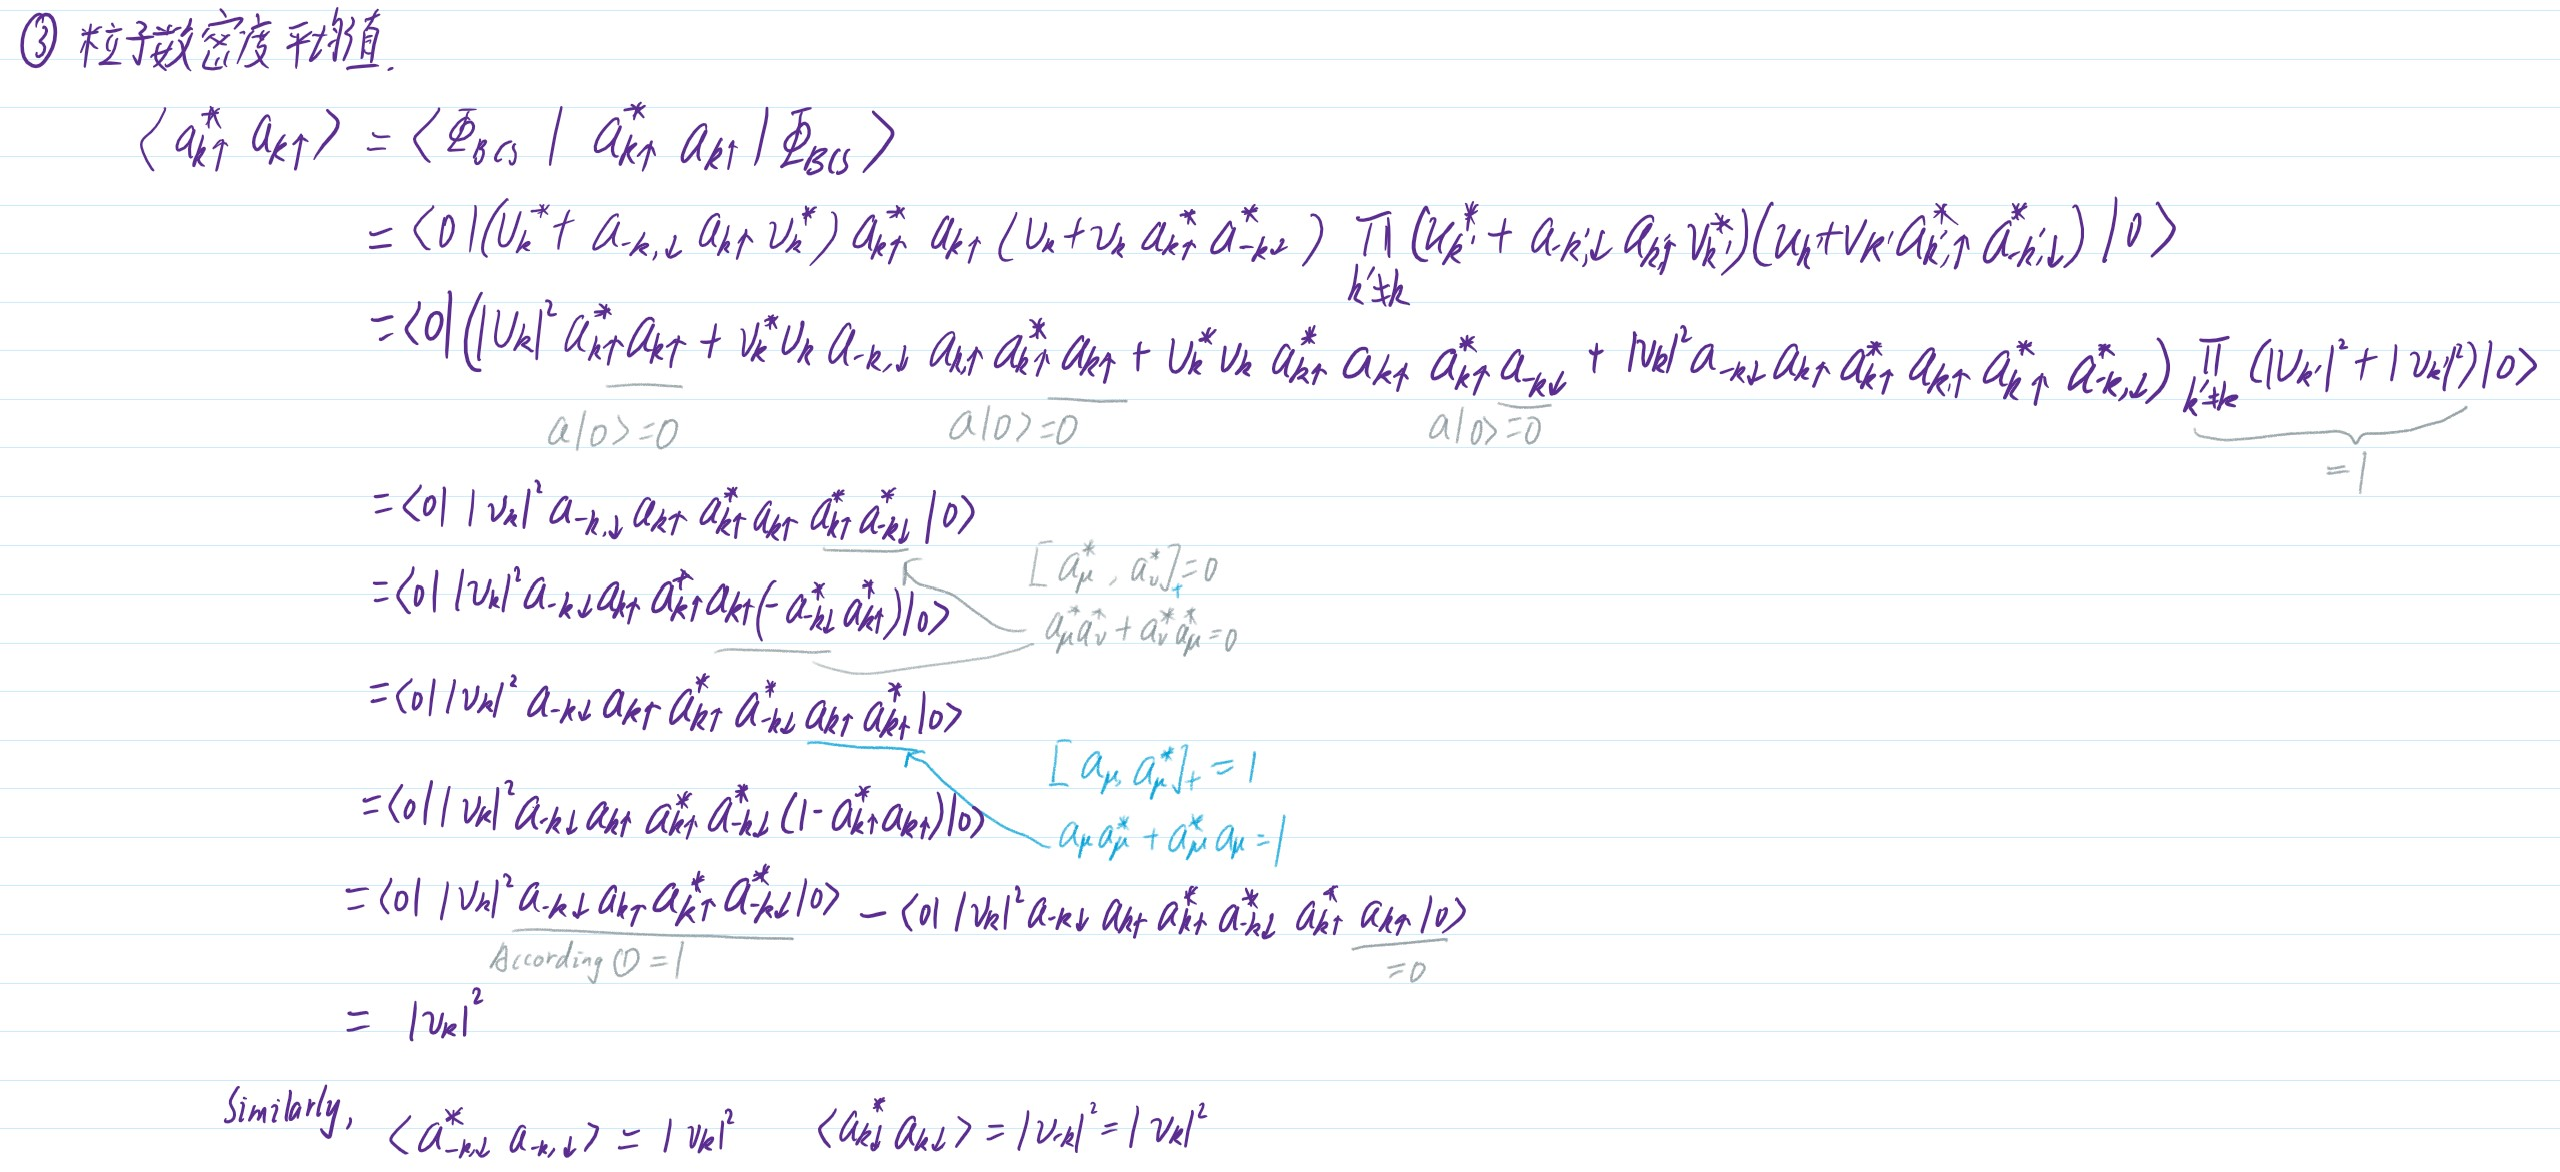
\includegraphics[scale=0.57]{Question/Task1-3.jpg}\\
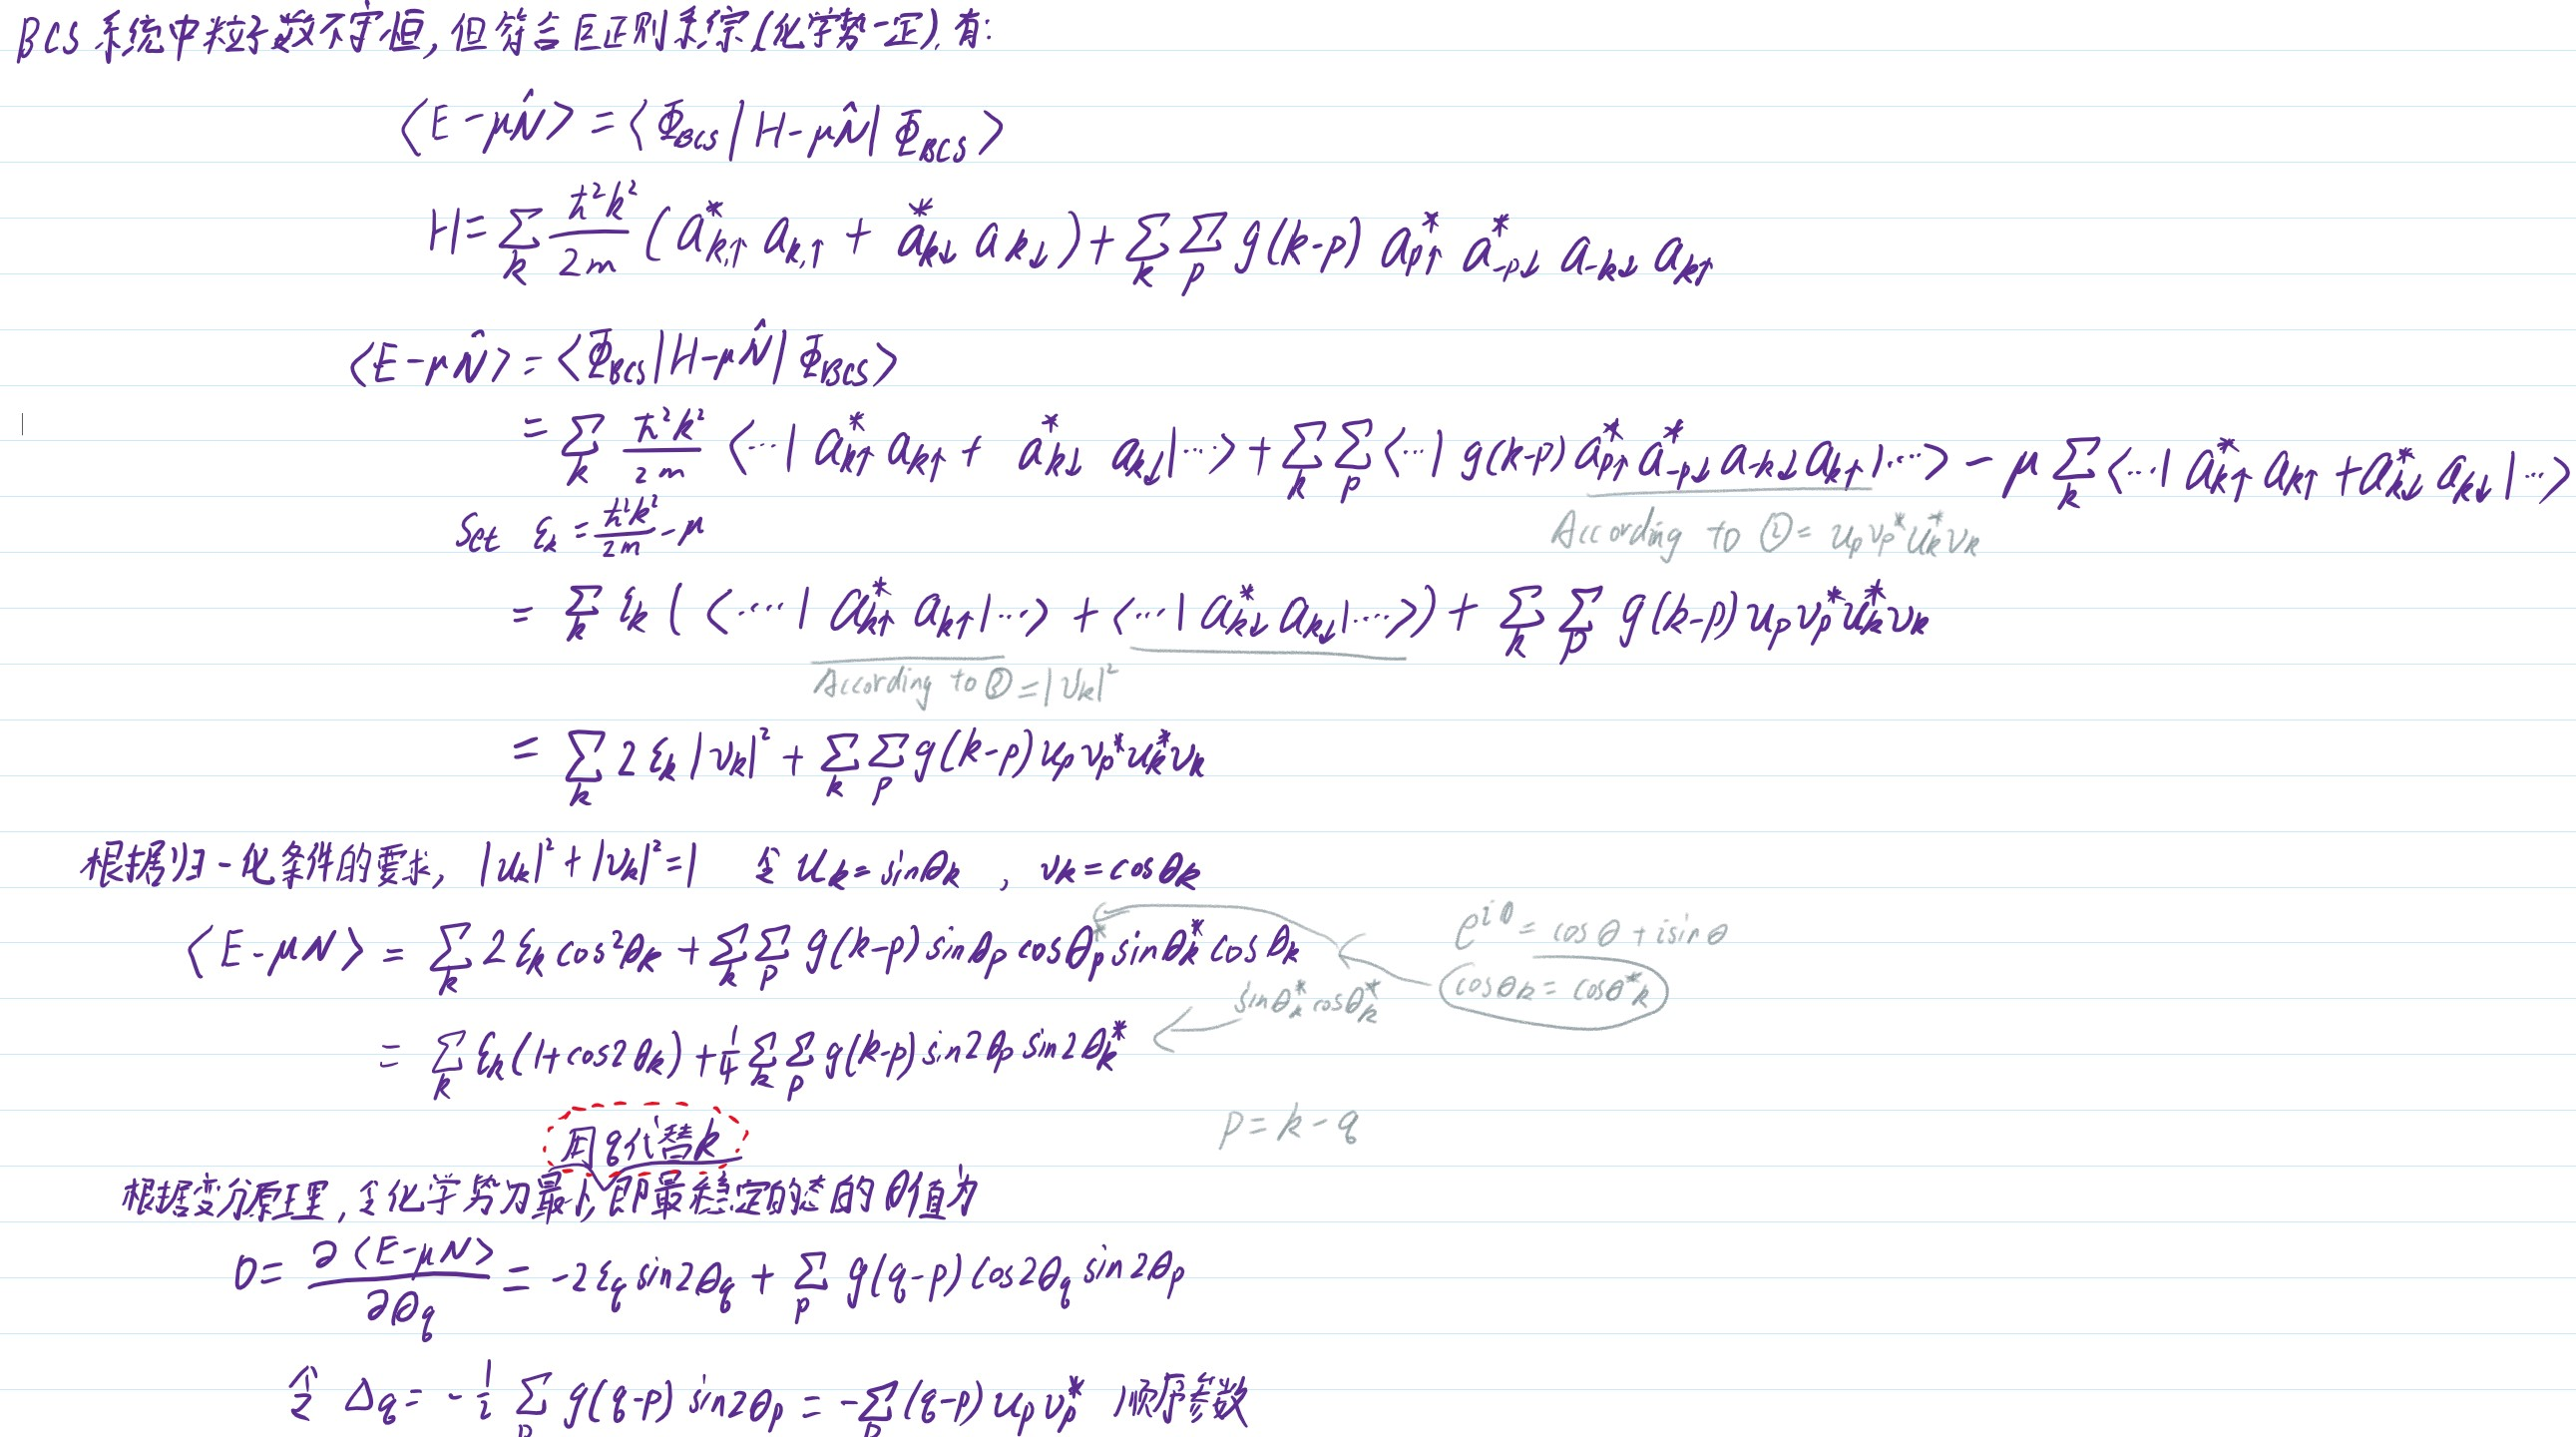
\includegraphics[scale=0.57]{Question/Task1-4.jpg}\\
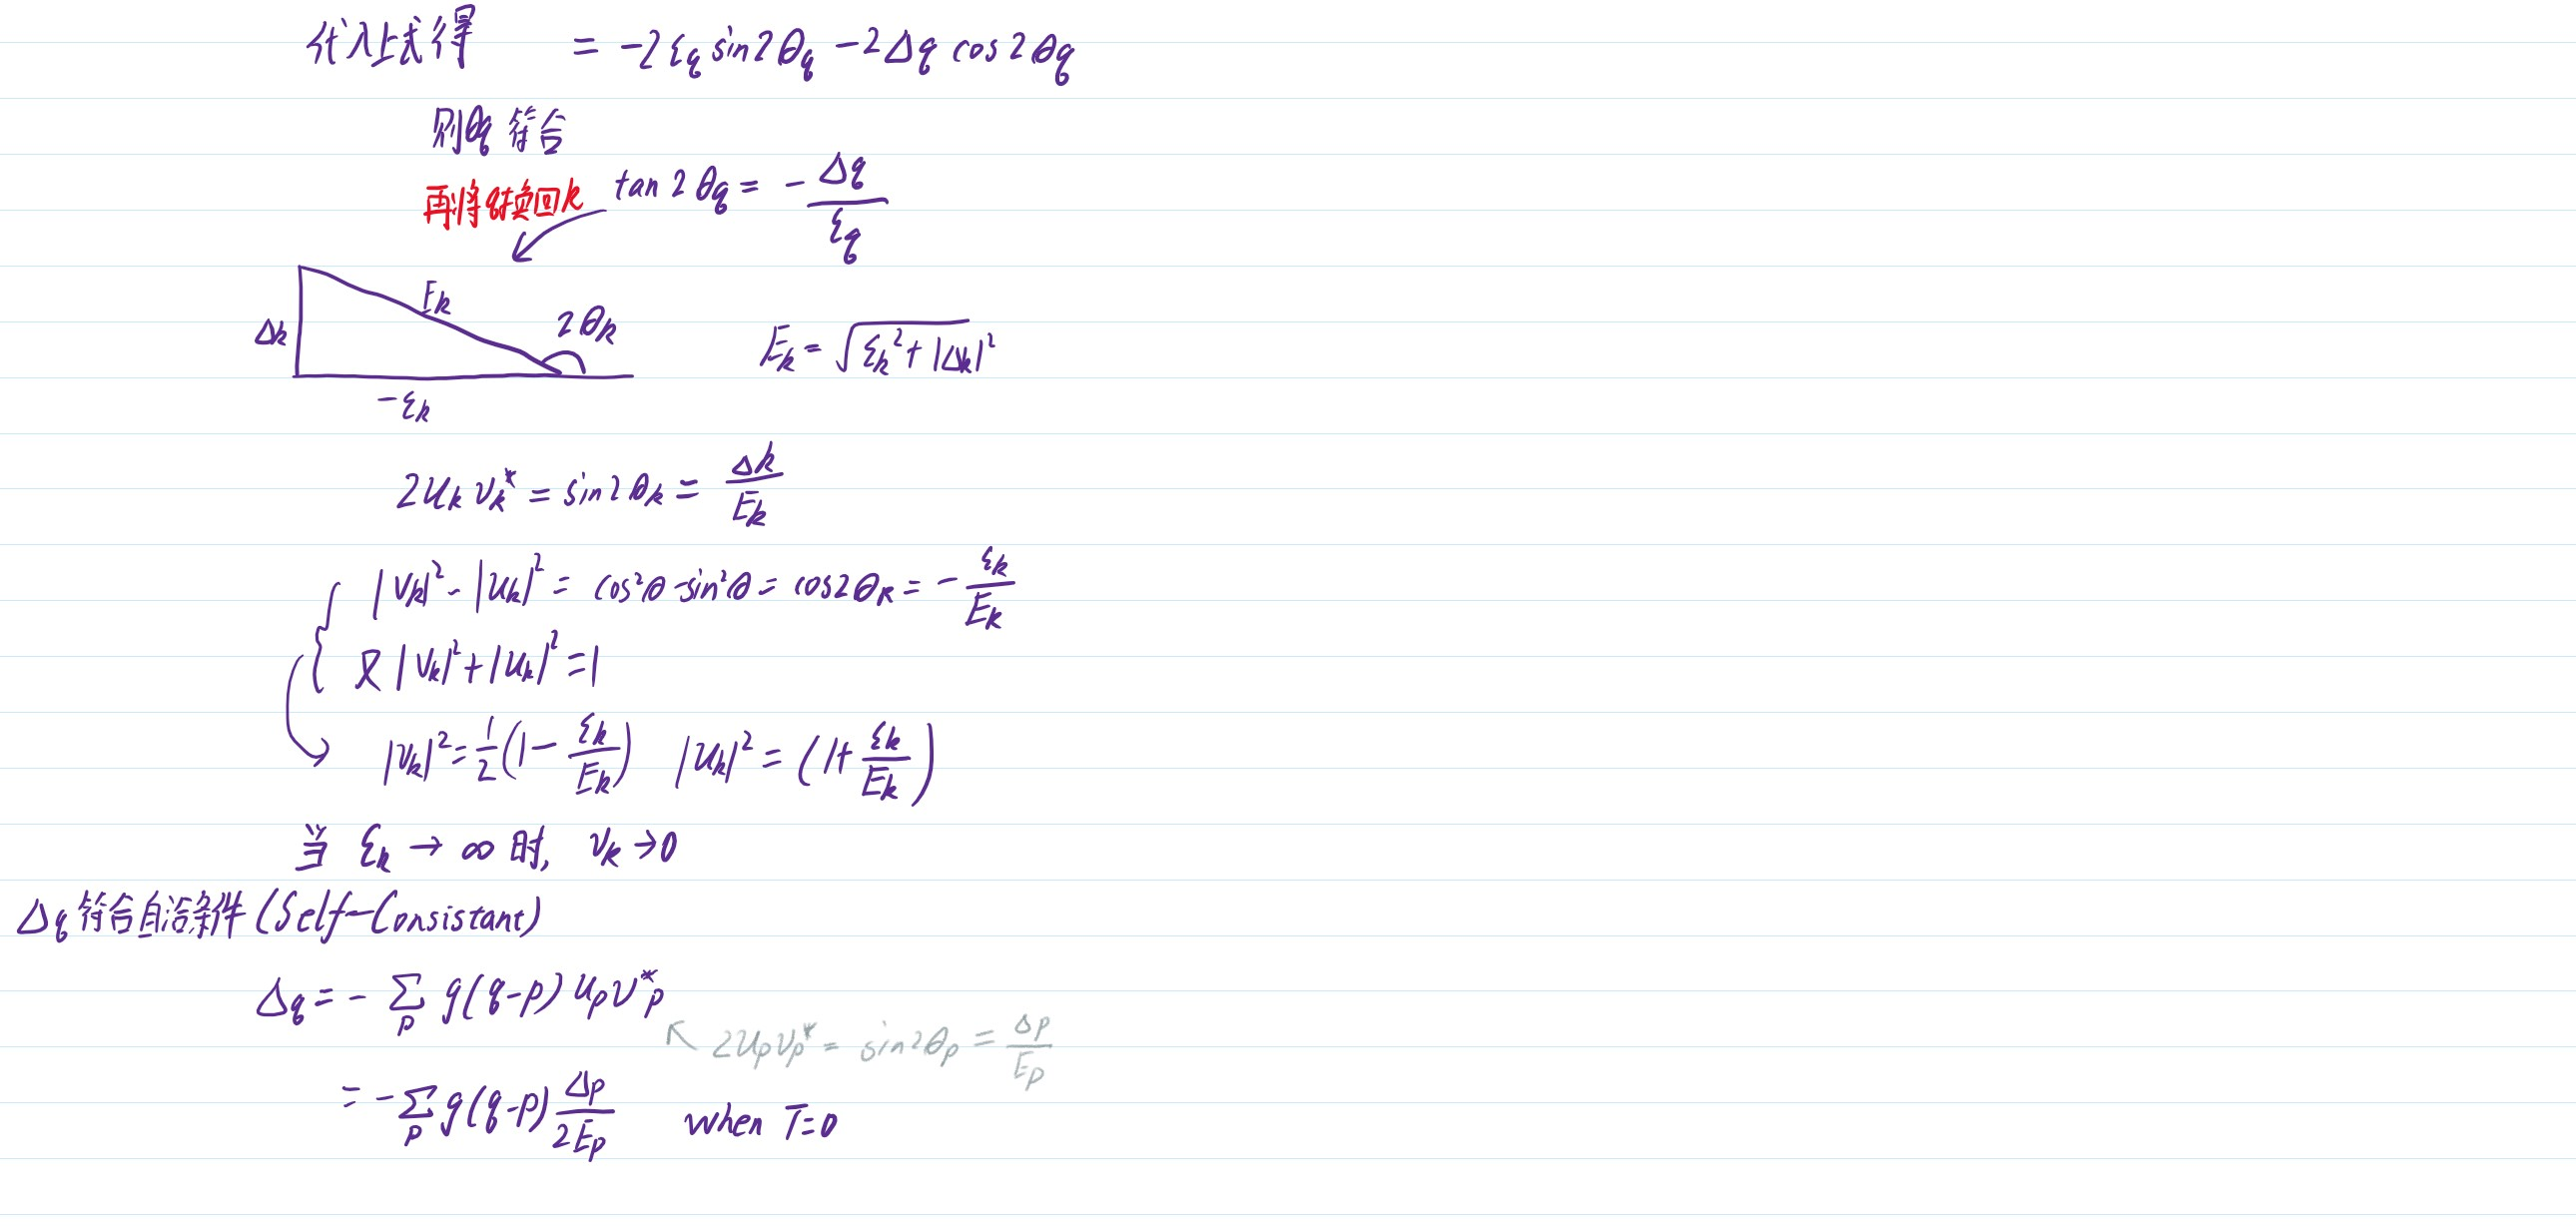
\includegraphics[scale=0.57]{Question/Task1-5.jpg}\\
\end{document}
